%!TEX root = ../main.tex 
\section{Efficient algorithms}
\label{sec:fast}
\subsection{The numerical cost of adaptive windows}

In the three last sections, we presented two adaptive windows algorithms that significantly improved over state-of-the-art algorithms, both theoretically and experimentally. Yet, our numerical experiments indicate that these improvements are computationally expensive. Indeed, at each round $t$, we store, update and compare $\cO\pa{t}$ statistics. 

The full update of the statistics can be done at a worst case cost of $\cO\pa{t}$. Indeed, each statistics $\hmu_i^h$ can be refreshed with a $\cO\pa{1}$ operation: 
\[\hmu_i^{h+1}(n+1) = \frac{h}{h+1}\hmu_i^{h}(n) + \frac{1}{h+1}o_t \,. \]

The comparison part in both \FEWA and \RUCB is also a $\cO\pa{t}$ operations. In \FEWA , we do a scan based on $\hmu_i^{h}$ for all $i \in \arms_h$ with increasing $h$. Hence, the total number of unitary operations is in $\cO\pa{t}$ in the worst case, as it scales with the number of statistics. \RUCB computes one UCB for each of the $\cO\pa{t}$ statistics. For each arm, it selects the minimum UCB as the index, which can be done with complexity $\cO\pa{t}$. Finally, finding the largest index is a $\cO\pa{K}$ operation. Therefore, we can conclude,

\begin{proposition}
At any round $t$, \FEWA and \RUCB have a $\cO\pa{t}$ worst-case complexity in time and memory.
\end{proposition}

\begin{remark}
\SWA($h$) has a $\cO\pa{h}$ worst-case complexity in time and memory because the sliding-window mechanism needs to store and update $\cO\pa{h}$ statistics to always have the average of the $h$ last sample ready. Hence, when it is optimally tuned for the minimax bound, $\SWA$ has a $\cO\pa{T^{2/3}}$ per round complexity. As often in non-stationary bandits, it may be possible to replace sliding window statistics with discounted statistics. Such modification often leads to a slightly worse theoretical regret rate with a much better $\cO\pa{K}$ complexity. 
\end{remark}

Hence, handling a large number of windows, which is the main strength of our algorithms to achieve a lower regret, is a significant drawback when it comes to design fast algorithms. Therefore, it is an open question whether one can enjoy the benefits of adaptive windows without suffering large time and space complexity. 

\subsection{The efficient update trick}
We detail \EFF, an update scheme to handle efficiently statistics of different windows. A similar yet different approach has appeared independently in the context of streaming mining~\citep{bifet2007learning}. \EFF is built on two main ideas: \emph{geometrically sparse} and \emph{delayed} statistics.

First, at any time $t$ we can avoid using $\left\{\hmu_i^h\right\}_{h}$ for all possible windows $h$ starting from 1 with an increment of 1. In fact, both statistics $\hmu_i^h$ and constructed confidence levels $c(h, \delta_t)$  have very close value for successive $h$ as $h$ becomes large: 
\begin{align*}
& \hmu_i^{h+1}(n) = \hmu_i^{h}(n) + \cO\pa{\frac{\sigma + L}{h}}\,,\\
& c(h+1, \delta_t) = c(h, \delta_t) + \cO\pa{\frac{\sigma }{h^{3/2}}} \,.
\end{align*}
Hence, in both \FEWA and \RUCB, we compute a lot of very similar quantities. Instead, we could use fewer statistics which are significantly different: $\left\{\hmu_i^h(\Nitmonepi)\right\}_{h\in \Him}$, where the window $h$ is dispatched on a geometric grid, 
 \[\Him\pa{\Nitmonepi} \triangleq \left\{ h_j \in  \left\{1, \dots , \Nitmonepi \right\} \;|\; h_{j+1} = \ceil{m \cdot h_j} \text{ and } h_1 = 1\right\}\quad \text{with } m > 1.\]

When there is no confusion, we drop the dependency on $\Nitmonepi$.  This modification alone is not enough to reduce both the time and space complexity. Indeed, updating $\hmu^h_{i}$ requires to replace the $h$-th last sample by the new one $o_t$. Hence, we need to store the $t$ collected samples to be able to update any $\hmu^h_{i}$  with $\cO\pa{1}$ complexity. Therefore, in \EFF, we will use $\cO\pa{K\log\pa{t}}$ \emph{delayed} statistics that we can update with $\cO\pa{K\log\pa{t}}$ space and time complexity.

\EFF (Alg.~\ref{alg:effupdate}) takes as input the new observation $o_t$ that the learner gets at the $N_i$-th pull of arm $i$; the geometric window grid $\Him$ tuned with an hyperparameter $m>1$, and for each window $h_j$ in this grid, three different numbers $\hmueff,\; \peff, \; \neff$. $\left\{\hmueff\right\}_{i,h_j}$ represents the set of \emph{current} statistics of window size $h_j$ that will be used instead of $\left\{\hmu_i^h\right\}_{i,h}$ in our efficient algorithms. We also store a pending statistic $\peff$ and a count $\neff$  which are used in the sparse update procedure of $\hmueff$. \EFF outputs an updated set of statistics.  
\begin{figure*}[!ht]
\begin{minipage}{\textwidth}
\renewcommand*\footnoterule{}
\begin{savenotes}
\begin{algorithm}[H]
\caption{{\EFF}}
\label{alg:effupdate}
\begin{algorithmic}[1]
\Require $o_t$, \small $\Him \gets \left\{h_j \! <\! \ceil{m \cdot N_i} \; | \;  h_{j+1} \!=\! \ceil{m \cdot h_j}  \text{with } h_0 \!=\! 1\right\} $\normalsize, $\left\{ \{ \hmueff,\, \peff, \, \neff \}\right\}_{h_j \in \Him}$
\If{$N_i = \max\pa{\Him}$}\label{algline:effu-new-condition} \Comment{Create a new triplet with window $h_j = \ceil{m \cdot N_i}$}  
\State $\Him \gets \Him \cup \left\{ \ceil{m \cdot N_i} \right\}$\label{algline:effu-new-h}
\State $p_i^{\ceil{m \cdot N_i} } = p_i^{N_i} $\label{algline:effu-new-p}
\State $n_i^{\ceil{m \cdot N_i} } \gets n_i^{N_i} $\label{algline:effu-new-n}
\State $\hmu_{i, \, \tteff}^{\ceil{m \cdot N_i} }\leftarrow \texttt{None}$\label{algline:effu-new-mu}
\EndIf\label{algline:effu-new-end} 
\State $p_i^{1} \gets o_t$ \label{algline:effu-update-first-p} \Comment{Update the first triplet with $o_t$}
\State $n_i^{1} \gets 1$\label{algline:effu-update-first-n}
\State $\hmu_{i, \, \tteff}^{1}\leftarrow o_t$ \label{algline:effu-update-first-hmu}
\For{$h_j \in  \Him \smallsetminus \left\{ 1\right\} $}\label{algline:effu-update-start} \Comment{Update the other pending statistics $\peff$ and $\neff$}
\State $p_i^{h_j} \gets p_i^{h_j}  +o_t$\label{algline:effu-update-p}
\State $n_i^{h_j} \gets n_i^{h_j} + 1$\label{algline:effu-update-n}
\EndFor\label{algline:effu-update-end} 
\For{$h_j \in  $ \textsc{Sort\_Desc}$\pa{\Him \smallsetminus \left\{ 1\right\} }$}\label{algline:effu-refresh-start}
\If{$n_i^{h_j} = h_j$} \label{algline:effu-refresh-condition}
\State $\hmueff \leftarrow p_i^{h_j}/h_j$ \Comment{Replace the current statistic $\hmueff$}\label{algline:effu-refresh-hmu}
\State{$p_i^{h_{j}} = p_i^{h_{j-1}} $} \label{algline:effu-refresh-p}\Comment{Refresh the pending statistics}
\State $n_i^{h_{j}} \gets n_i^{h_{j-1}} $\label{algline:effu-refresh-n}
\EndIf
\EndFor \label{algline:effu-refresh-end}
\Ensure $\left\{\left\{  \hmueff,\; p_i^{h_j}, \; n_i^{h_j} \right\}\right\}_{h_j \in \Him}$
\end{algorithmic}
\end{algorithm}
\end{savenotes}
\end{minipage}
\end{figure*}
The core of \EFF is divided in four parts: 1) From Lines~\ref{algline:effu-new-condition} to~\ref{algline:effu-new-end}, we create new window's statistics at a logarithmic rate with respect to the growth of $N_i$; 2) From Lines~\ref{algline:effu-update-first-p} to~\ref{algline:effu-update-first-hmu}, we update the statistics of window $h_1=1$;
3) From Lines~\ref{algline:effu-update-start} to~\ref{algline:effu-update-end}, we update the other pending statistics and count;
4) From Lines~\ref{algline:effu-refresh-start} to~\ref{algline:effu-refresh-end}, we eventually update $\hmueff$ and refresh the corresponding pending statistic and count. The remaining details are quite technical. Thus, we first give the high-level properties that are ensured by the recursive usage of \EFF. Then, we prove them by going through the algorithm line by line.\newpage

\begin{proposition}
\label{prop:effu}
 $\left\{\left\{  \hmueff,\; p_i^{h_j}, \; n_i^{h_j} \right\}\right\}_{h_j \in \Him}$, constructed recursively with \EFF with initial value $\left\{\left\{  \hmu_{i,\,\tteff}^1 : \texttt{None},\; p_i^{1} :0 , \; n_i^{1}:0 \right\}\right\}$ have the following properties:
 \begin{enumerate}[topsep=0pt]
  \item $\hmueff$ is the average of exactly $h_j$ consecutive samples among the $2h_j -1$ last ones. \label{list:effu-hmu}
  \item The delay between two updates of $\hmueff$ is in $\left\{\ceil{\frac{m-1}{m} h_j}, \dots, h_j -1\right\}$.\label{list:effu-delay}
%  \item When $m = 2$, $h_j = 2^{j}$. Moreover, for $j\geq1$,  the $k$-th update $\hmueff$ happens at pull $ \pa{k+1} \cdot 2^{j-1}$, \ie every $2^{j-1}$ pulls (and at every rounds for $j=0$).\label{list:effu-m2}
  \item $\peff$ is the sum of the $\neff$ last samples. \label{list:effu-p}
  \item $\neff < h_j$ for $j\geq 1$. Also, $n_i^1 \leq 1$.\label{list:effu-n1}
  \item $\left\{ \neff \right\}_{h_j}$ is an non-decreasing sequence with respect to $h_j$ (or $j$).\label{list:effu-n2}
 \end{enumerate}
\end{proposition}
\begin{proof}
The three last properties are trivially true at the initialization. Thus, we show by induction that they remain true after updates.
\paragraph{Proof of \ref{list:effu-p}. } At Lines~\ref{algline:effu-new-p} and~\ref{algline:effu-new-n}, we create a new pending statistics and count by initializing them with other statistics and counts. Hence, because of the recursion hypothesis, all the pending statistics $\peff$ (including the created one) contains the sum of the $\neff$ \emph{before last} pulls. At Lines~\ref{algline:effu-update-first-p} and~\ref{algline:effu-update-first-n}, we update $p_i^1$ with the last sample and set $n_i^1$ to $1$. At Lines~\ref{algline:effu-update-p} and~\ref{algline:effu-update-n}, we add the last sample to $\peff$ (which was containing the before last samples) and increase the count by $1$. Hence, at the end of Line~\ref{algline:effu-update-n}, all the $\peff$ contains the sum of the last $\neff$ samples. Thus, refreshing $\peff$ and $\neff$ with $ p_i^{h_{j-1}}$ and $n_i^{h_{j-1}}$ keeps this property true (Lines~\ref{algline:effu-refresh-p} and~\ref{algline:effu-refresh-n}). 

\paragraph{Proof of \ref{list:effu-n1}.}
For $j=0$, $n_i^1$, which is equal to $0$ at the initialization, is set at $1$ at every update (Line~\ref{algline:effu-update-first-n}). Hence, we have $n_i^{h_0} \leq h_0=1$.
For $j\geq 1$, $n_i^{\ceil{m \cdot N_i}}$ is initialized at Line~\ref{algline:effu-new-n} with the value $n_i^{N_i} < N_i < \ceil{m \cdot N_i}$ by the induction hypothesis and because $m>1$.  Then, $\neff < h_j$ ($j\geq1$) is increased by one at each update at Line~\ref{algline:effu-update-n}. Hence, we now have $\neff \leq  h_j$ for all $j\in\Him$. However, for $j\geq 1$, if $\neff = h_j$ (Line~\ref{algline:effu-refresh-condition}), it is replaced by the precedent count $n_i^{h_{j-1}}\leq h_{j-1} < h_j$ (Line~\ref{algline:effu-update-n}). Thus, at the end of the update, we do have $\neff < h_j$ for $j\geq1$.

\paragraph{Proof of \ref{list:effu-n2}.}
At Line~\ref{algline:effu-new-n}, we create a new pending count corresponding to the largest $h_j$ and we initialize it with the precedent largest count. At Lines~\ref{algline:effu-update-first-n} and~\ref{algline:effu-update-n}, we set $n_i^1 =1$ and increase all the other $\neff$ by one. This operation preserves the non-decreasing property of the ordered set. Last, at Line~\ref{algline:effu-refresh-n}, we set few counts $\neff$ to the precedent value $n_i^{h_{j-1}}$- which also preserves the non-decreasing property of the ordered set. 

\paragraph{Proof of \ref{list:effu-hmu} and \ref{list:effu-delay}.}
Thanks to Property~\ref{list:effu-p}, we know that $\peff$ is the sum of the $\neff$ last sample. It is still true at the end of Line~\ref{algline:effu-update-n} (see the proof). Then, at Line~\ref{algline:effu-refresh-hmu}, and given the condition in Line~\ref{algline:effu-refresh-condition}, we set $\hmueff$ with the average of the last $h_j$ sample. Then, $\hmueff$ is not updated untill the condition at Line~\ref{algline:effu-refresh-condition} is fulfilled again. 

$\neff$ is refreshed with a quantity larger or equal to $1$ and smaller or equal to $h_{j-1}$ at Line~\ref{algline:effu-refresh-n}. Then, it is increased by one at each update. we know that $\hmueff$ will be updated at least every $h_j-1$, and at most every $h_j -h_{j-1}$ round. Hence, considering the worst possible delay we can conclude: $\hmueff$ is the average of exactly $h_j$ consecutive samples among the $2h_j -1$ last ones. Last, considering that $h_{j-1}\leq h_j /m$, we conclude that the minimal delay is larger or equal to $\frac{m-1}{m}h_j$.
\end{proof}

In Proposition~\ref{prop:effu-complexity}, we show that \EFFU succeeds to drastically reduce the time and space complexity of the updates as soon as $m$ is not too close to $1$.
\begin{proposition}
\label{prop:effu-complexity}
After $N_i$ updates, the time and space complexity of \EFFU scales with $\cO\pa{\min\pa{ \log_m{N_i}, N_i}} $.
\end{proposition}
\begin{proof}
The time and space complexity scales with $|\Him|$. Indeed, there are $3|\Him| + 2$ variables store in memory : $\left\{ \{ \hmueff,\, \peff, \, \neff \}\right\}_{h_j \in \Him}$, $o_t$ and $N_i$. Moreover, \EFFU does two $\textsc{For}$ loops on $\Him$.

The size of $\Him$ is upper-bounded by $\cO\pa{\log_m N_i}$. Indeed, when the condition at Line~\ref{algline:effu-new-condition} is fulfilled, $\max\pa{\Him}$ is replaced by $\ceil{m\cdot N_i}$. When it is not fulfilled, the maximum is not changed but $N_i$ increases by one unit. Hence, we always have, 
\[
\max\pa{\Him} \leq \ceil{m\cdot N_i}.
\]
Moreover, when the condition is fulfilled, the maximum is replaced by,
\[
\max\pa{\Him} \leftarrow \ceil{m \cdot\max\pa{\Him}}.
\]
Hence, when $\Him$ is initialized with $\left\{1\right\}$, we show recursively that, 
\[\max\pa{\Him} \geq m^{|\Him|-1}. \]
Combining the above equations, we have, 
\[m^{|\Him|-1} \leq m\cdot N_i +1. \]
Therefore, 
\[|\Him| \leq \log_m\pa{2N_i} + 2. \]
This upper-bound diverges at finite $N_i$ when $m\rightarrow 1$. However, the size of $\Him$ is increased one by one at Line~\ref{algline:effu-new-h}. Hence, even if the condition at Line~\ref{algline:effu-new-condition} is fulfilled at every round, $|\Him|\leq N_i +1$ ($\Him$ is initialized with $\left\{1\right\}$).
\end{proof}

\begin{remark}
When $m\leq 1 + \frac{1}{N_i}$, $\left\{\hmueff\right\}_{h_j \in \Him}$ (the outcome of \EFFU) is the same than the outcome of the classical update $\left\{\hmu_i^h\right\}_{h \leq N_i}$ for the $N_i$ first rounds. Yet, there is no free lunch, the complexity is $\cO\pa{N_i}$ in this regime (according to Proposition~\ref{prop:effu-complexity}).
\end{remark}



\subsection{The delay in {\EFF}}
We have already emphasized that \EFFU is built on two ideas: geometrically sparse and delayed statistics. The geometrically sparse aspect is straightforward to understand and quantify: $h_{j+1} \sim m \cdot h_j$ up to the rounding.

In this Subsection, we provide a tight analysis of the delay between the updates. In fact, the important quantity is the normalized delay, that is, the delay divided by the window size. Indeed, each statistic of window $h_j$ should represent the $h_j$ last sample. A delay of $10$ for $h_j = 10^6$ is very good as it succeeds to take into account most of the $h_j$ last sample. However, the same delay of $10$ is a failure when $h_j = 1$, as the algorithm fails to give a good representation of the very last sample.

In Property~\ref{list:effu-delay}, we show that the normalized delay cannot be larger than $100\%$. We also show that it is lower bounded by $\frac{m-1}{m}$. For small values of $m$, this amplitude can be large. 

We use two tricks in the algorithm to reduce the delay. First, at Line~\ref{algline:effu-refresh-n}, we refresh $\peff$ with $p_i^{h_{j-1}}$ which contains $n_i^{h_{j-1}} \in \left\{ 1, \dots, h_{j-1}\right\}$ samples. We could refresh $\peff$ and $\neff$ at $0$ which would lead to $100\%$ normalized delay. Instead, we use the variable available in the memory which contains the sum of $h$ last sample, with the largest $h< h_j$.  According to Properties~\ref{list:effu-p},~\ref{list:effu-n1} and~\ref{list:effu-n2}, this quantity is $p_i^{h_{j-1}}$. 

Indeed, according to Property~\ref{list:effu-p}, $p_i^{h_{j'}}$ contains the $n_i^{h_{j'}}$ last samples. At the round of the update of $\hmueff$,  $p_i^{h_{j'}}$ contains $h_j$ samples before Line~\ref{algline:effu-refresh-p}. According to Property~\ref{list:effu-n2}, all the $j'>j$ have  $n_i^{h_{j'}}>\neff = h_j$. According to Property~\ref{list:effu-n1}, $n_i^{h_{j-1}}\leq h_{j-1} < h_j$.  Moreover, for all $j' \leq j-1$, $n_i^{h_{j-1}} \geq n_i^{h_{j'}}$ (Property~\ref{list:effu-n2}).

The second trick is to sort $\Him$ in the decreasing order at Line~\ref{algline:effu-refresh-start}. If there are two synchronous consecutive updates of $\hmueff$ and $\hmu_{i,\, \tteff}^{h_{j+1}}$ at the same run of \EFF, doing a backward loop guarantees to refresh $n_i^{h_{j+1}}$ with $\neff = h_j$ instead of a smaller value if we would do a forward loop.

In this Subsection, we show that these two tricks succeed to upper-bound the normalized delay by $\cO\pa{\frac{m-1}{m}}$ when $m$ is an integer and when $m < 2$.


\subsubsection{The integer case.}
\begin{proposition}
\label{prop:effu-delay-int}
When $m \in \NN \setminus \left\{ 0, 1\right\}$,  $h_j = m^j$. Moreover, $\hmueff$ is updated periodically with period $\omega_j = \frac{m-1}{m} h_j$ for $j\geq1$ ($\omega_0 =1$).
\end{proposition}


The main idea is simple: since any window $h_j$ is a multiple of the lower order $h_{j-k}$, $\hmueff$ is initialized and updated synchronously with all the lower order statistics. Hence, the pending statistic $\peff$ is refreshed with $h_{j-1}$ sample, the largest possible number of sample in $p_i^{h_{j-1}}$. Hence, choosing integer values minimizes the delay (compared to the delay bounds we identify in Property~\ref{list:effu-delay}). The proof is quite technical, and we delay it at the end of the Subsection. 

\begin{figure*}[ht]
\centering
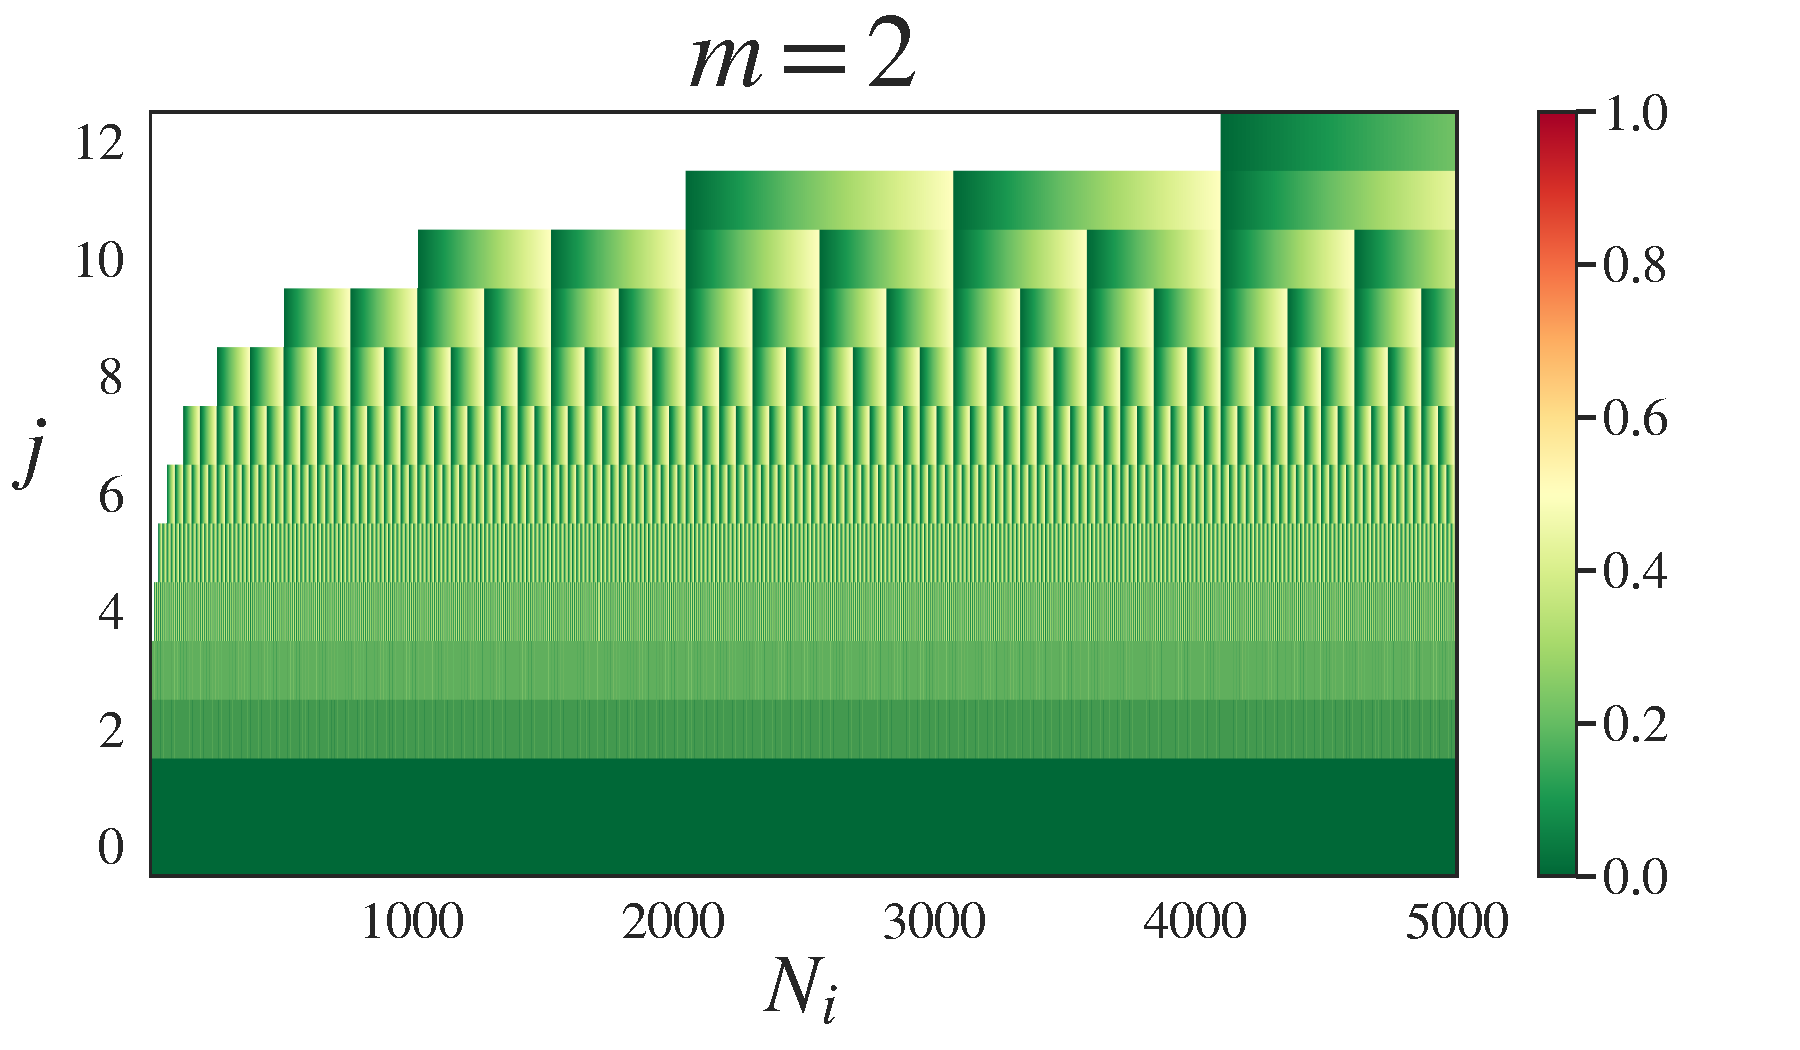
\includegraphics[clip, width= 0.49\textwidth]{2.1Rested/fig/T=5000_m=2.pdf}
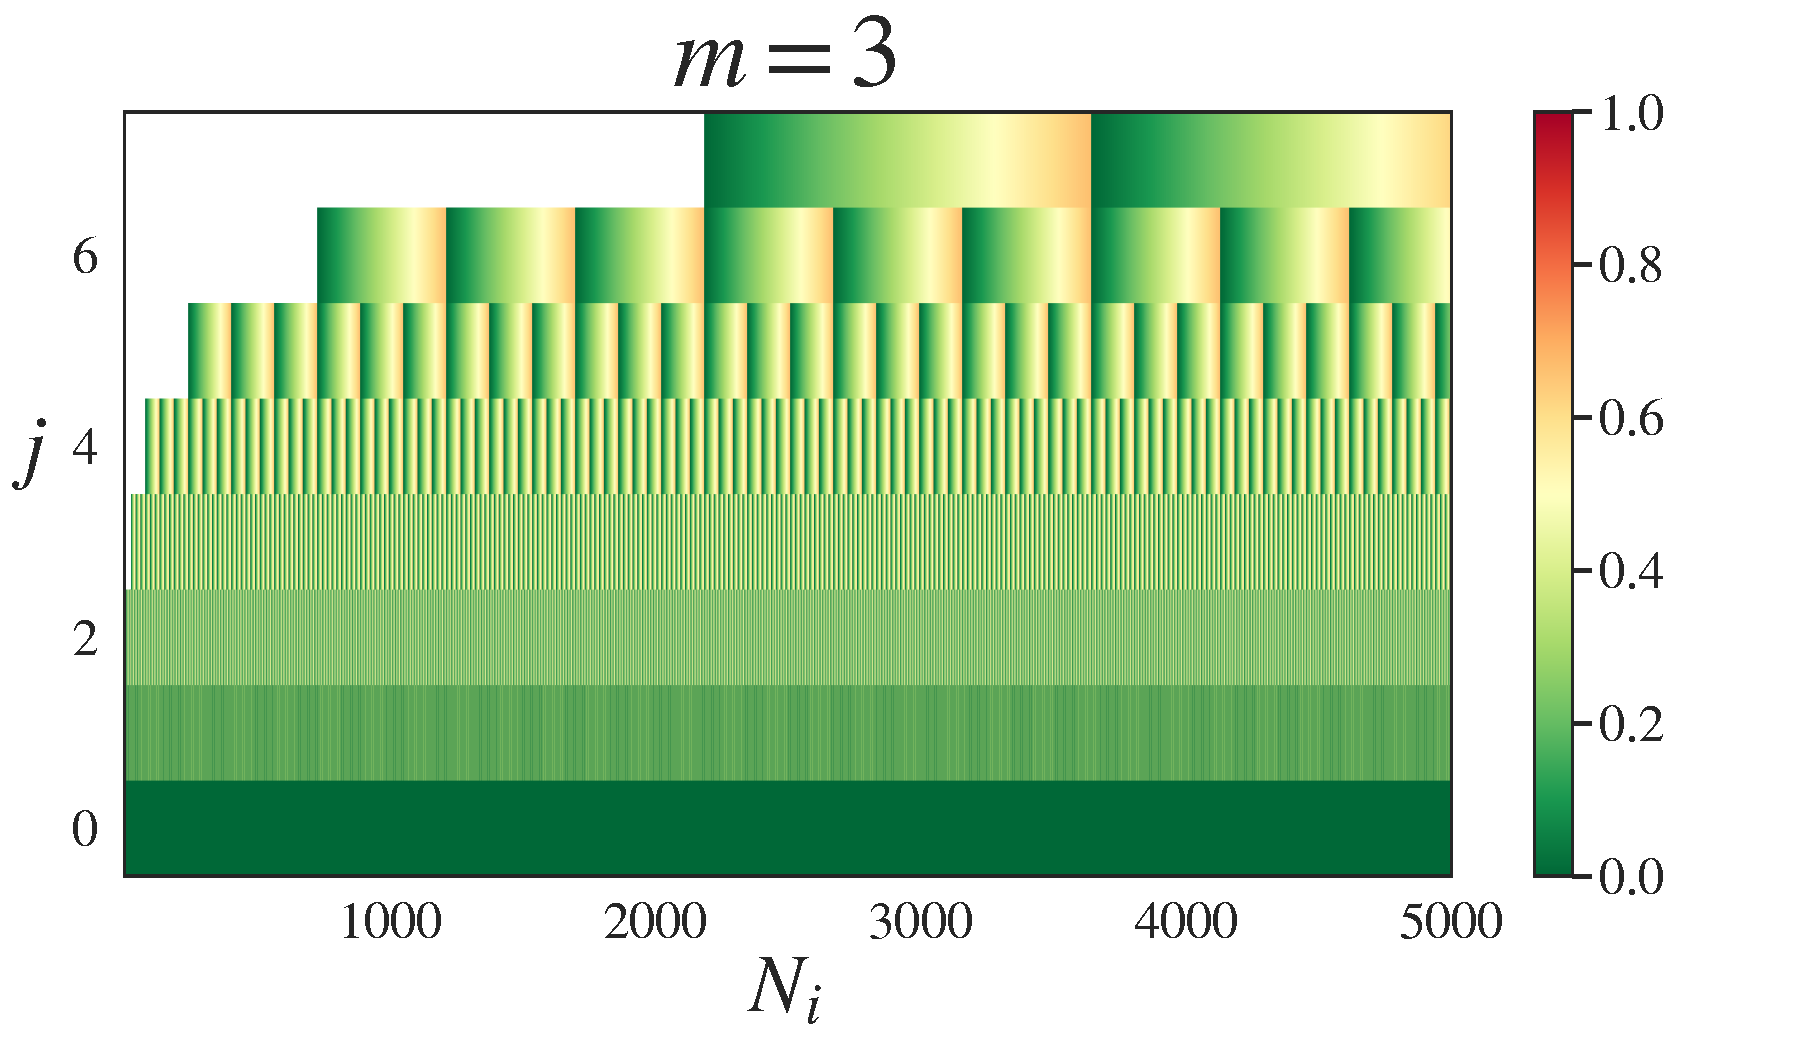
\includegraphics[clip, width= 0.49\textwidth]{2.1Rested/fig/T=5000_m=3.pdf}
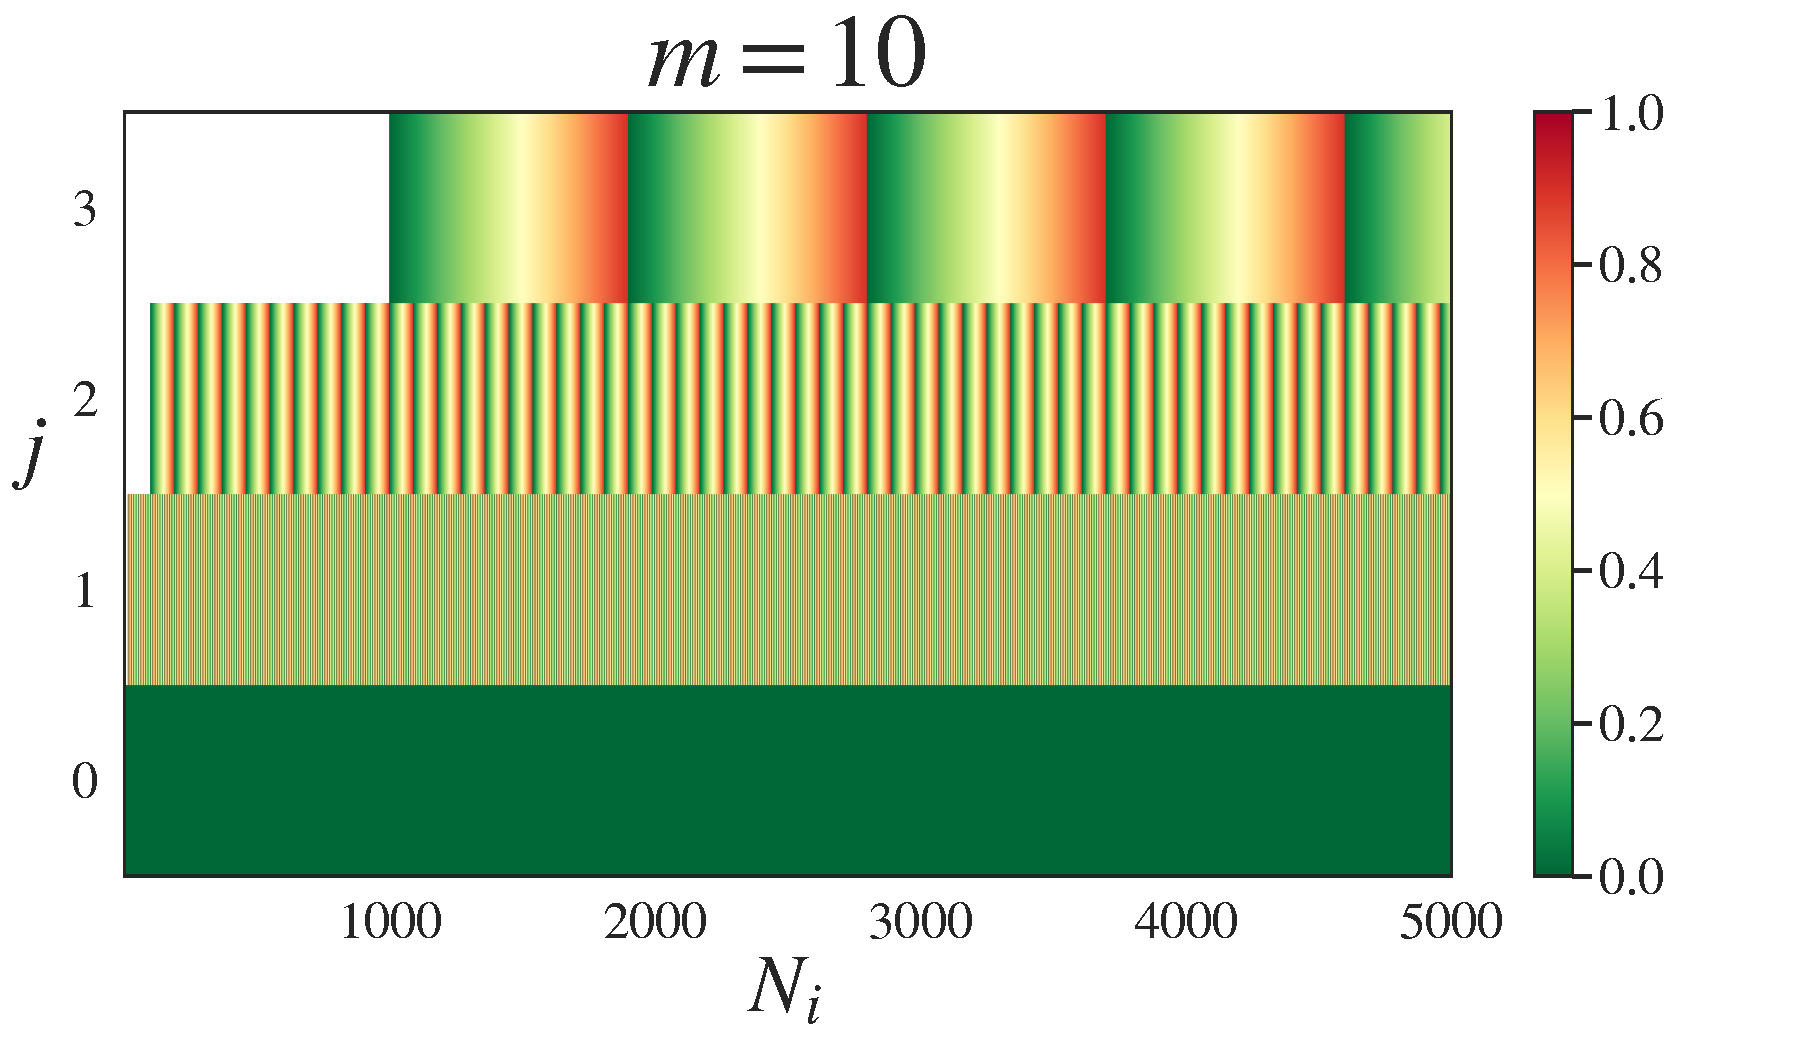
\includegraphics[clip, width= 0.49\textwidth]{2.1Rested/fig/T=5000_m=10.pdf}
\caption{Normalized delay $\nicefrac{d_j}{h_j}$ after $N_i$ pulls for each$j$-th statistic $\hmueff$. We display in white the rounds at which statistic $j$ is not created yet.}
\label{fig:delay-int}
\end{figure*}

We call $d_j(N_i) \in \left\{0, \dots, \omega_j-1 \right\}$, the number of pulls since the last update of statistic $\hmueff$ after $N_i$ pulls. We display in Figure~\ref{fig:delay-int}  
the normalized delay $\nicefrac{d_j}{h_j}$ after $N_i$ pulls of each statistic. The updates are indeed periodic. We notice the strong synchronization in the updates: not only each period $\omega_j$ is at a $m$ factor of the previous one, but the update of statistic $j$ are at the same round as the updates of statistics $j'<j$. %Figure.

However, for large values of $m$, the delay improvement is marginal. For $m=10$, each statistic can be delayed by $90\%$ their window size. Even, for $m=2$ the normalized delay $\nicefrac{\omega_j}{h_j}$ is $50\%$. The $\nicefrac{m-1}{m}$ ratio would be very interesting for $m \rightarrow 1$. 

\subsubsection{The non integer case}
\begin{figure*}[ht]
\centering
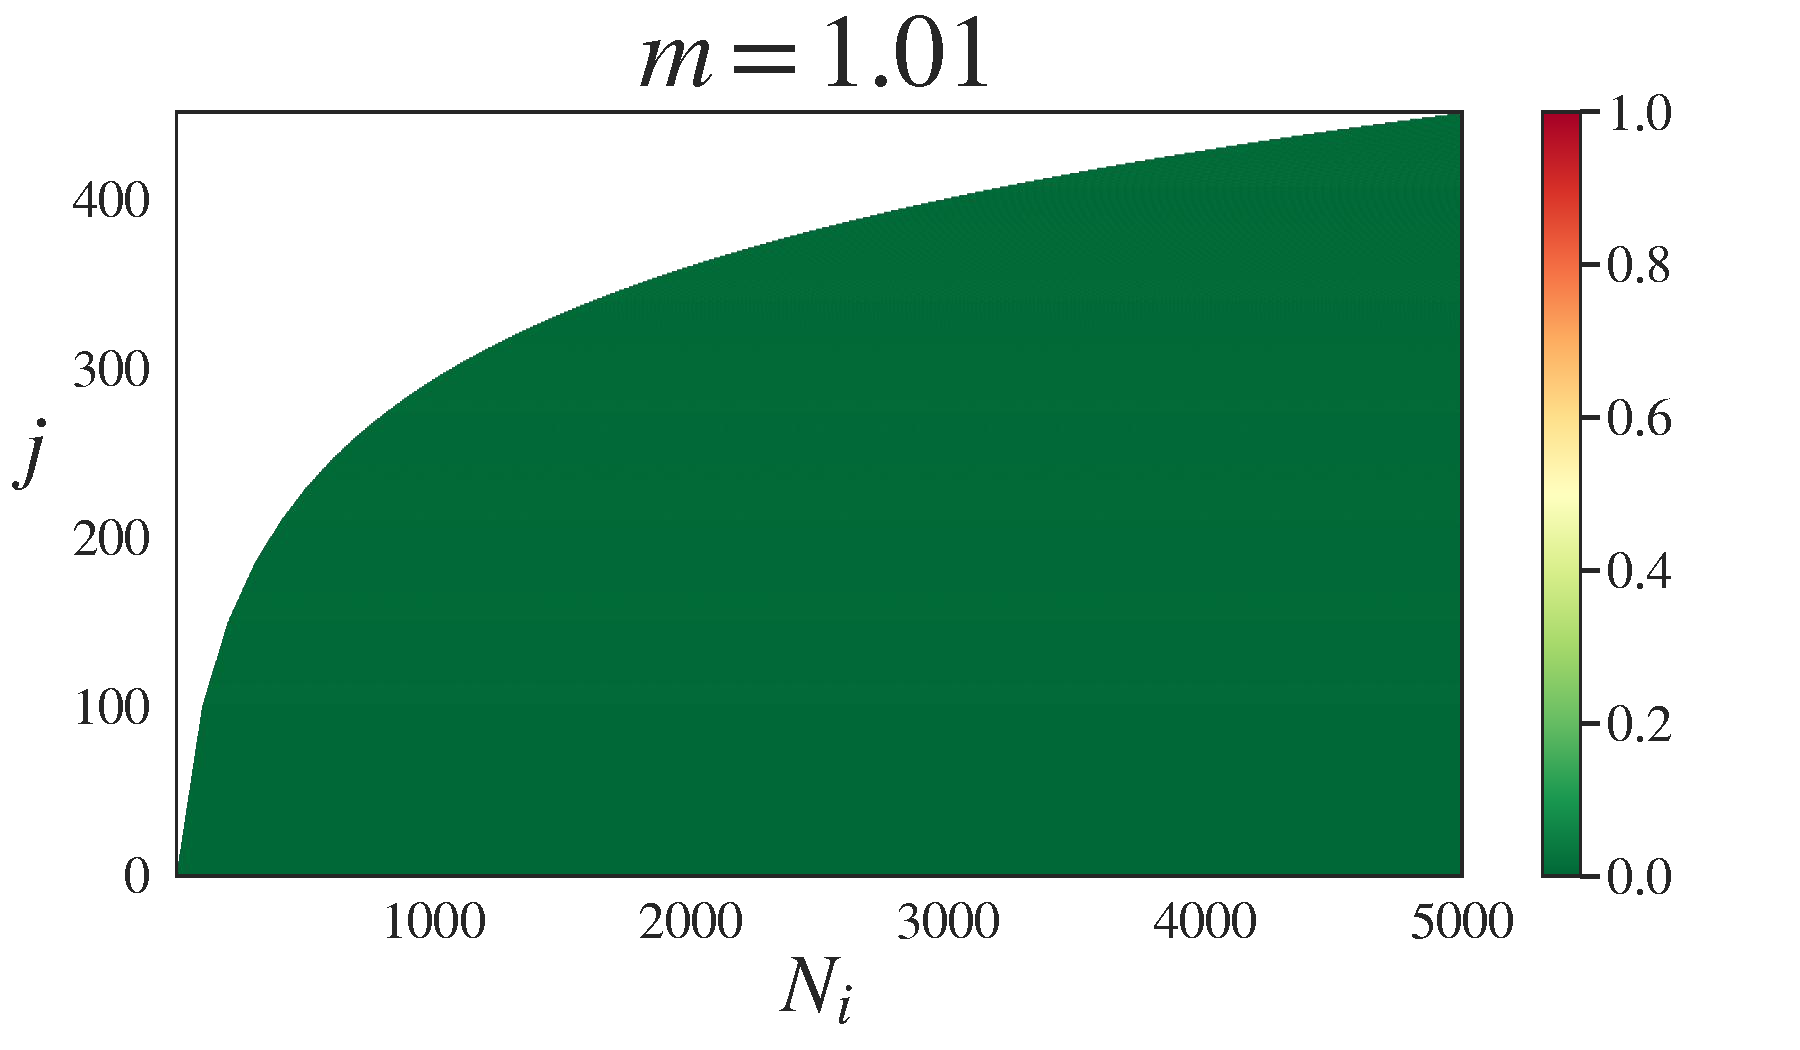
\includegraphics[clip, width= 0.325\textwidth]{2.1Rested/fig/T=5000_m=1,01.pdf}
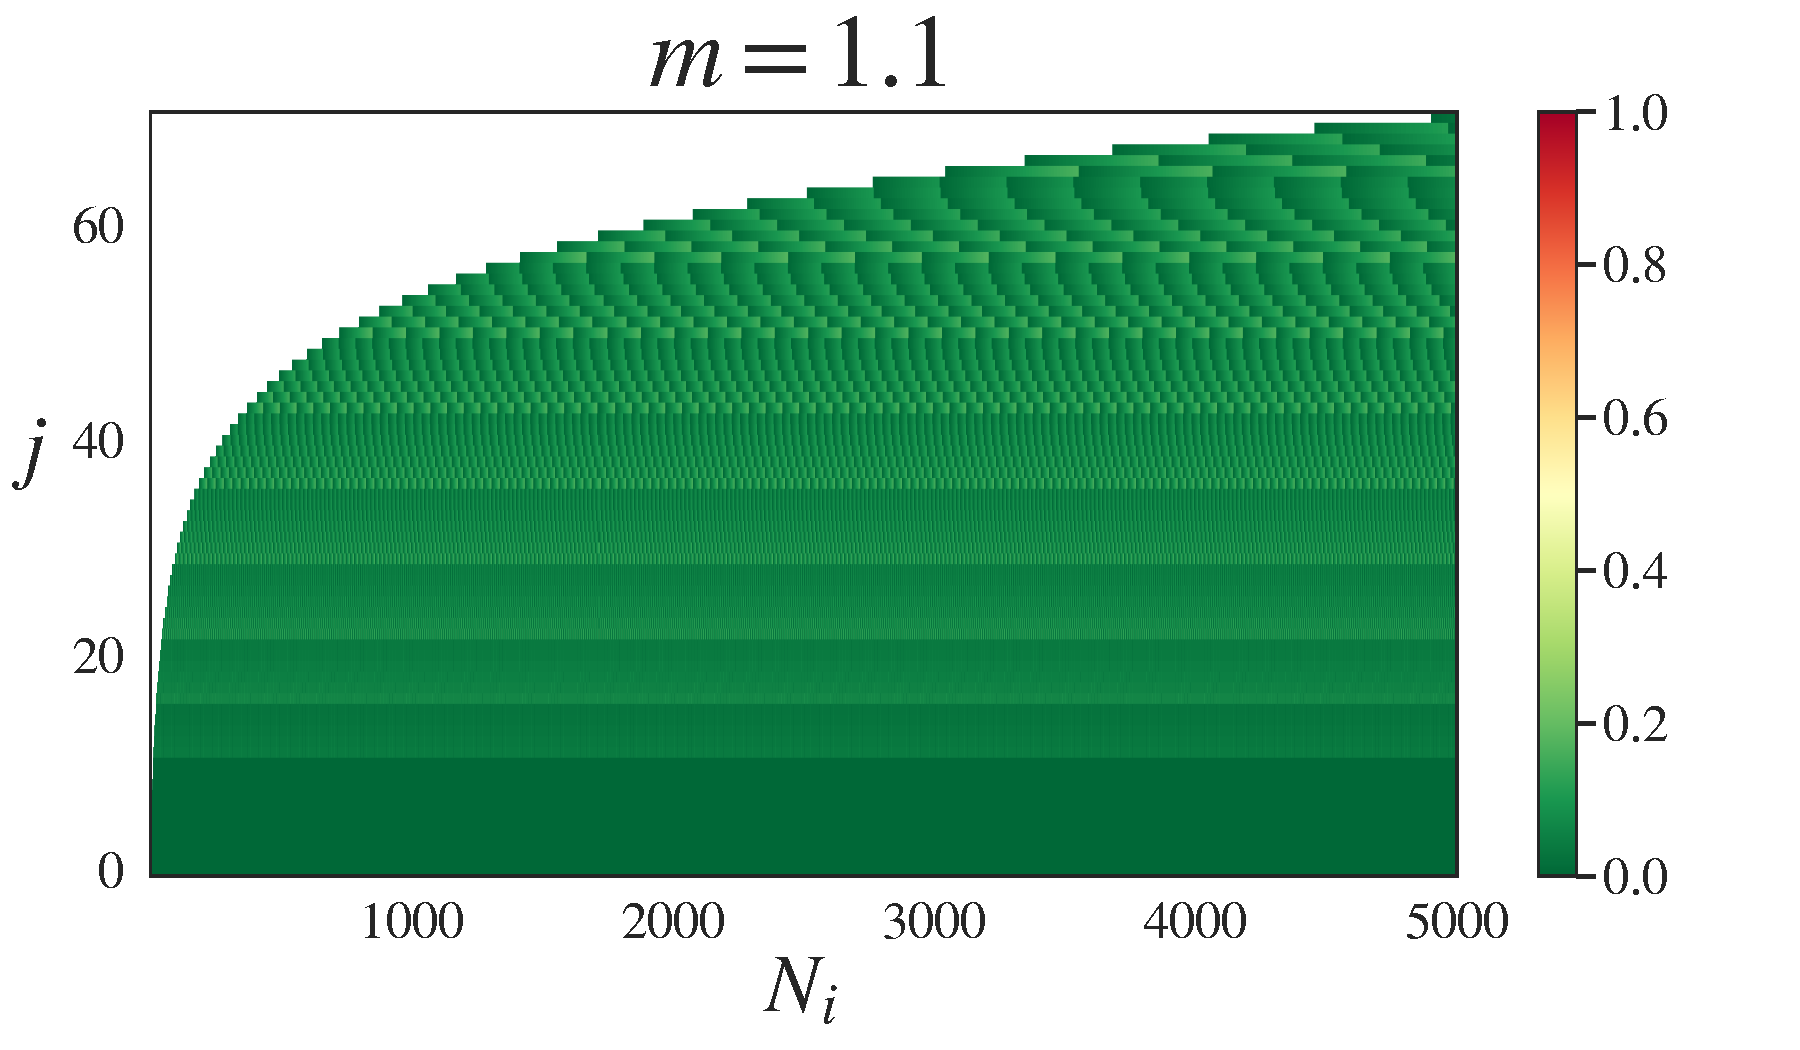
\includegraphics[clip, width= 0.325\textwidth]{2.1Rested/fig/T=5000_m=1,1.pdf}
%\includegraphics[clip, width= 0.325\textwidth]{2.1Rested/fig/T=5000_m=1,2.pdf}
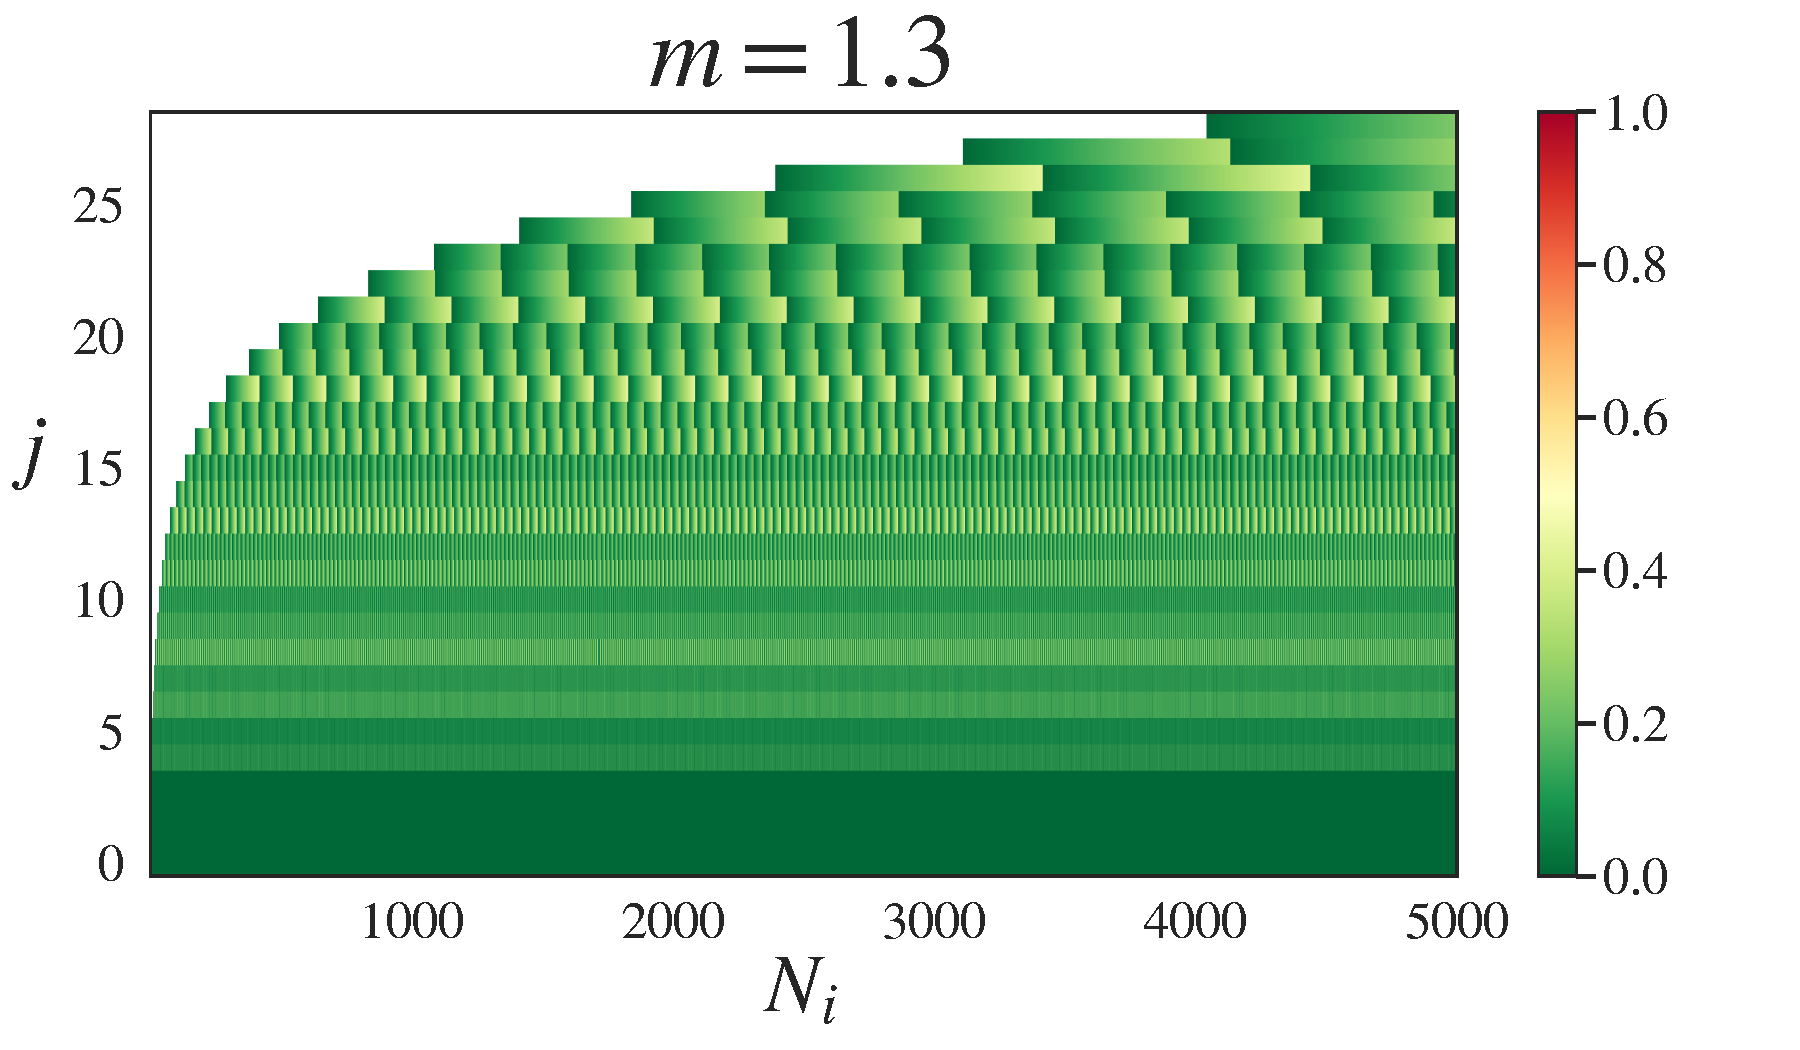
\includegraphics[clip, width= 0.325\textwidth]{2.1Rested/fig/T=5000_m=1,3.pdf}
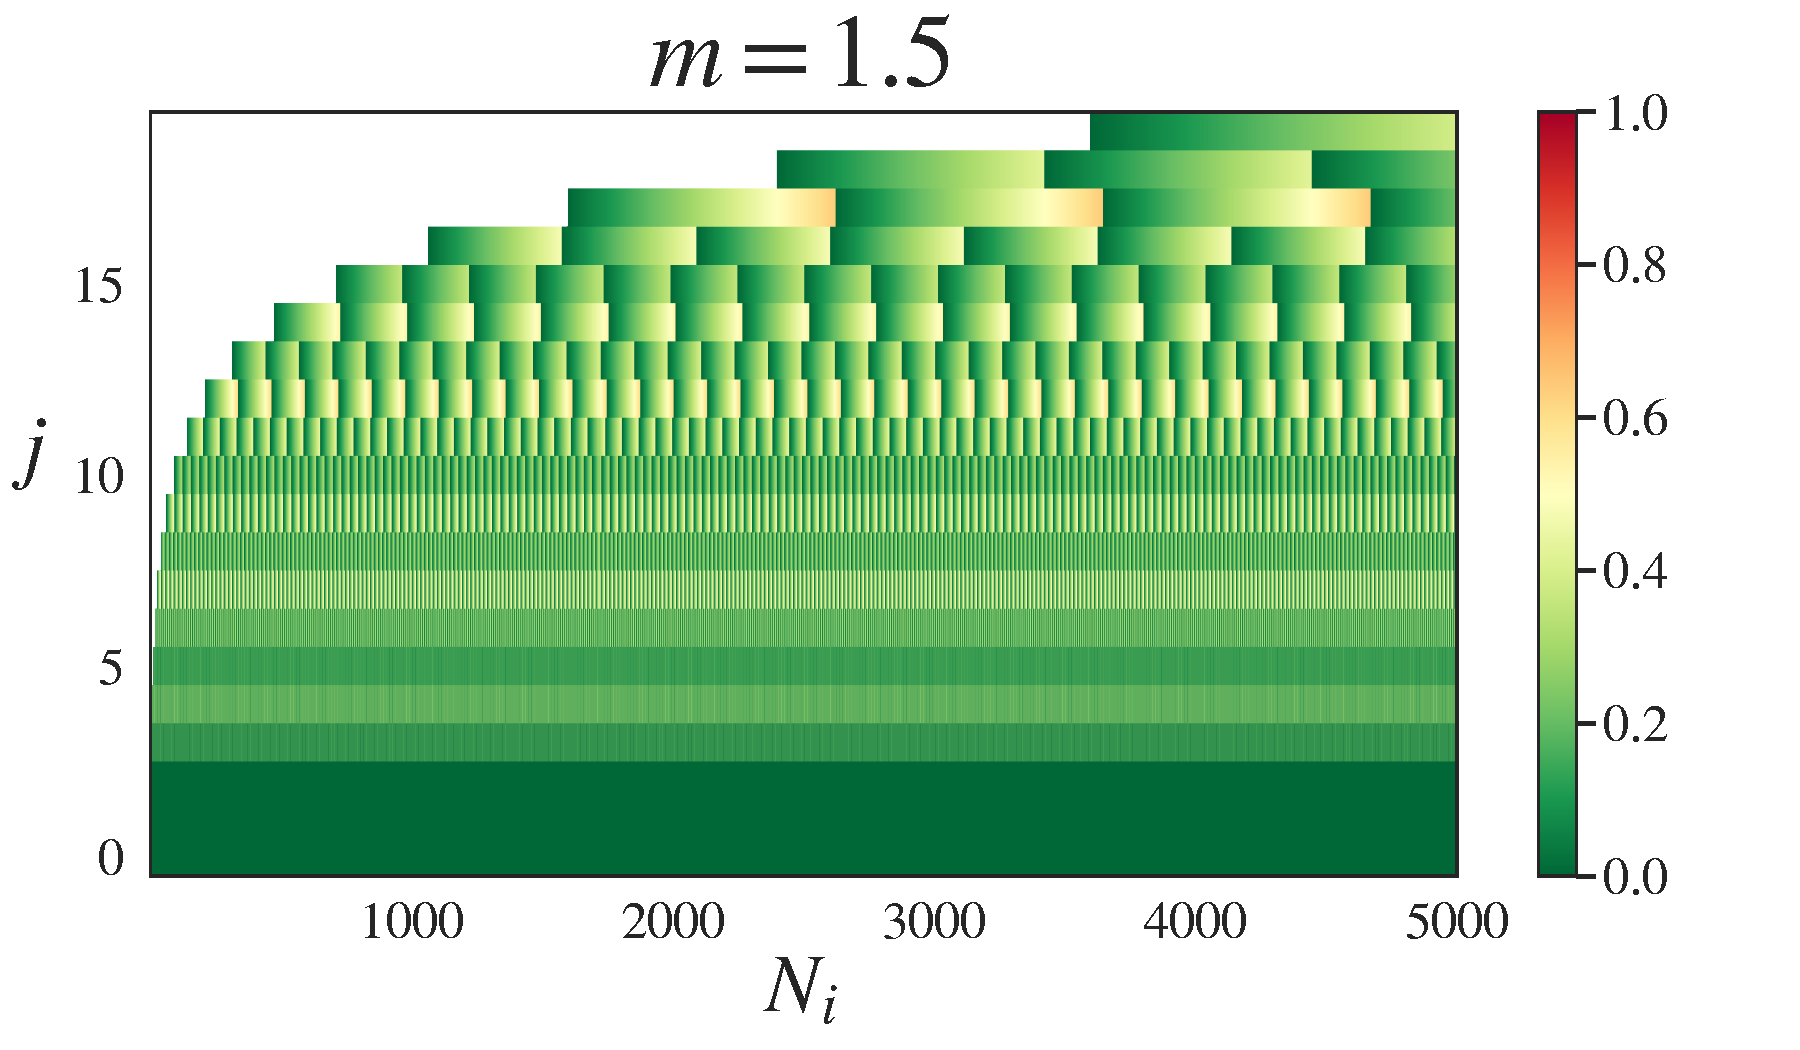
\includegraphics[clip, width= 0.325\textwidth]{2.1Rested/fig/T=5000_m=1,5.pdf}
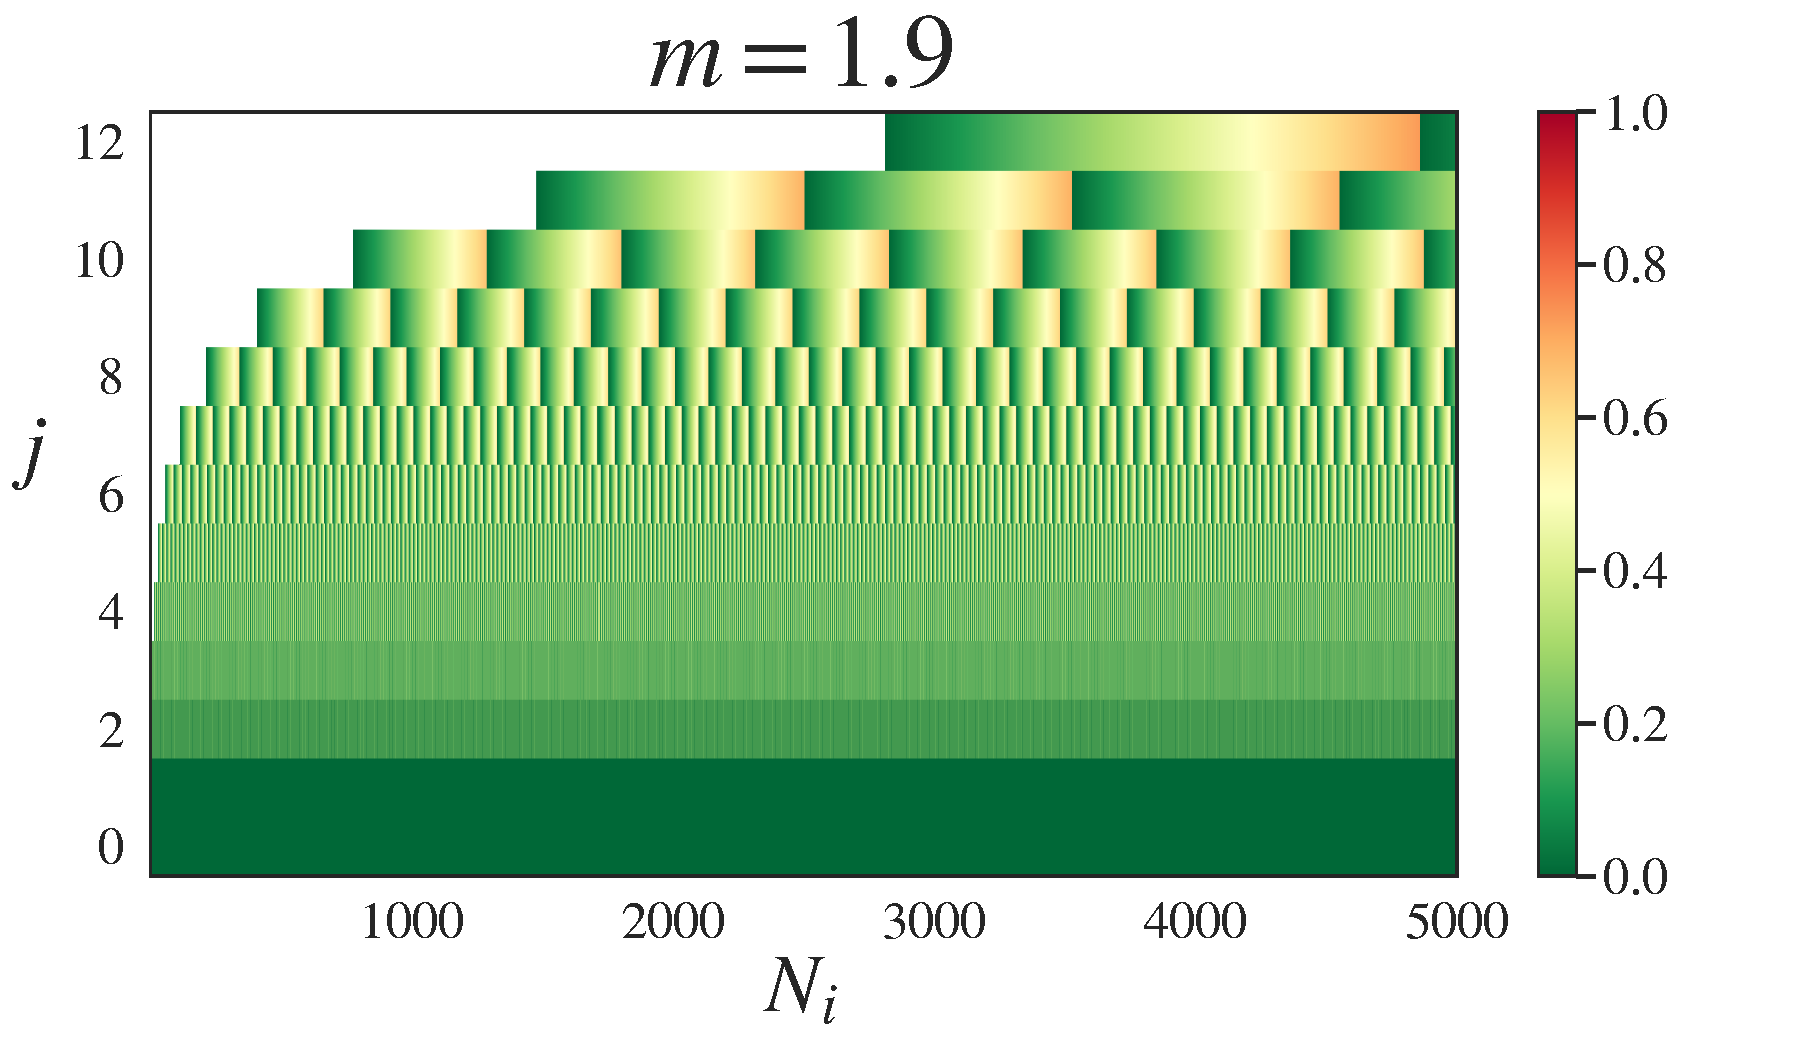
\includegraphics[clip, width= 0.325\textwidth]{2.1Rested/fig/T=5000_m=1,9.pdf}
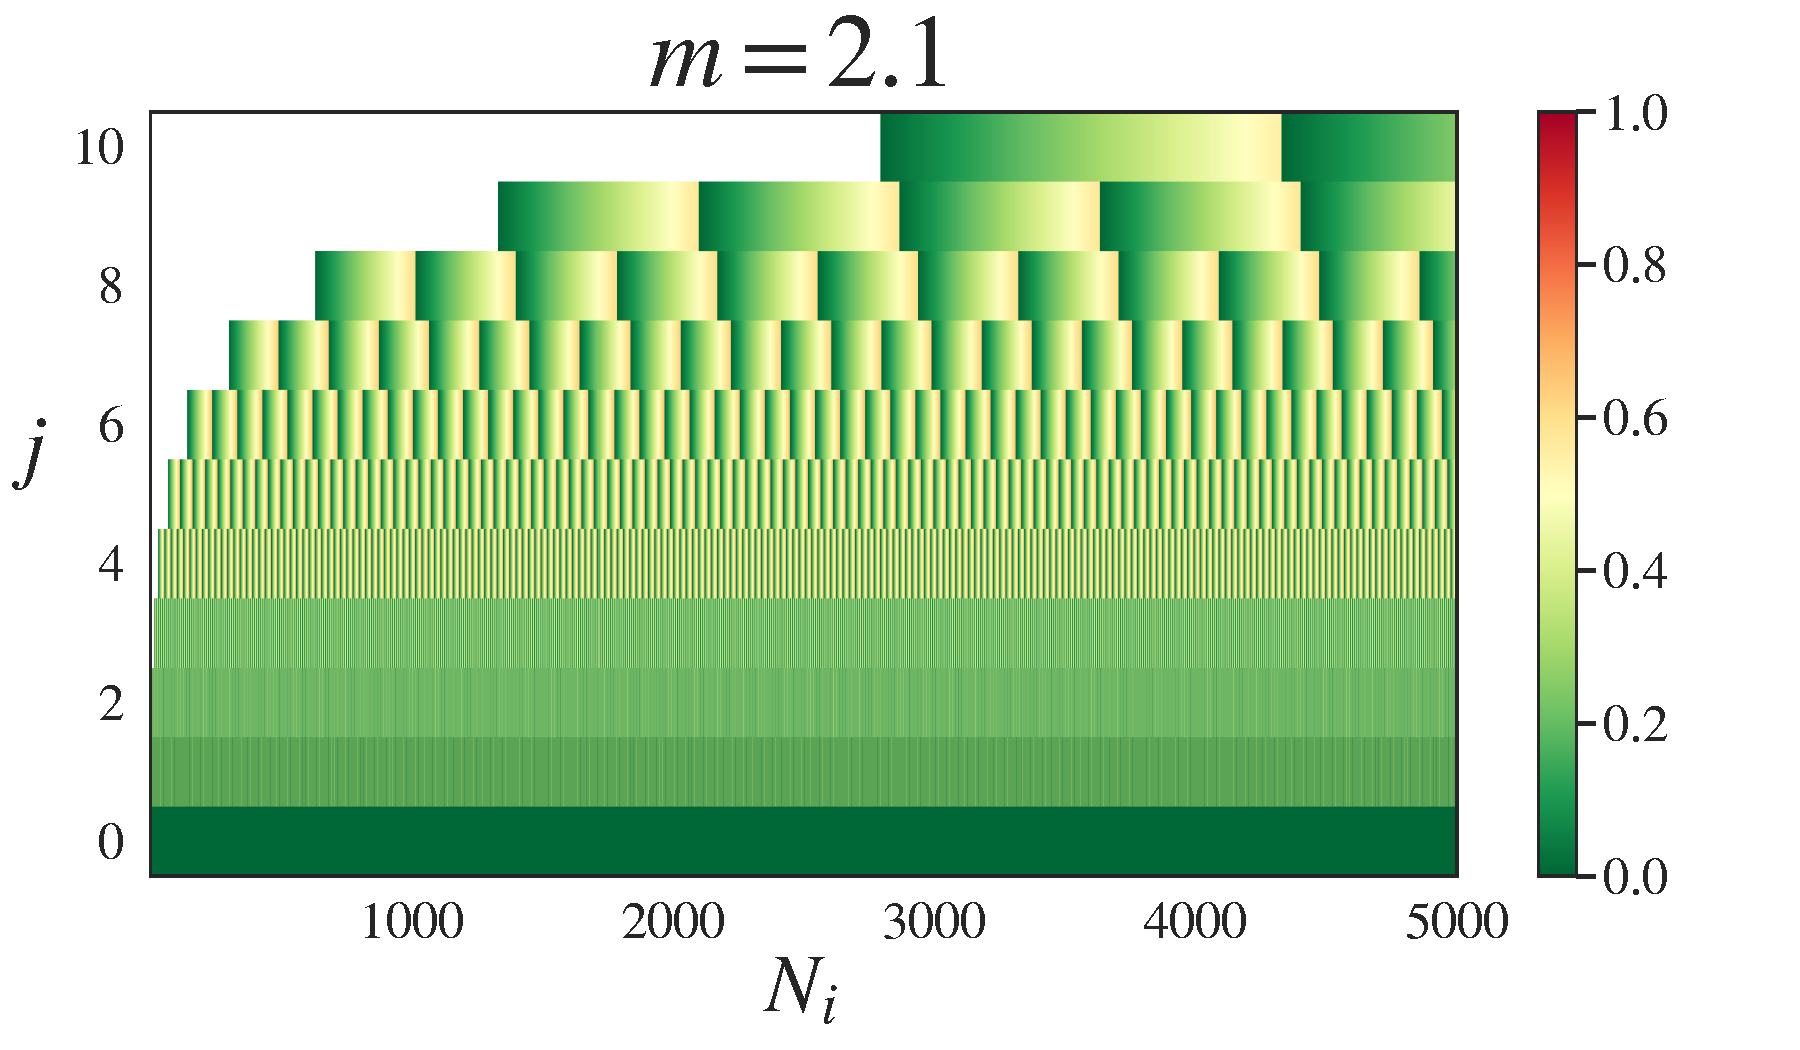
\includegraphics[clip, width= 0.325\textwidth]{2.1Rested/fig/T=5000_m=2,1.pdf}
\caption{Normalized delay $\nicefrac{d_j}{h_j}$ after $N_i$ pulls for each $j$-th statistic $\hmueff$. We display in white the rounds at which statistic $j$ is not created yet.}
\label{fig:delay-general}
\end{figure*}

In Figure~\ref{fig:delay-general}, we display the delay for several non integer values. Compared to the integer case, the update of statistic $j$ does not happen at the same round as the update of statistic $j'<j$. However, we notice that the updates are still periodic and the updating period $\omega_j$ is a multiple of $\omega_{j-1}$. We formalized this properties in Propositions~\ref{prop:effu-delay-periodic} and~\ref{prop:effu-delay-m2} which we show at the end of the Subsection. 

\begin{proposition}
\label{prop:effu-delay-periodic}
For each statistic, the updates are periodic. Moreover, the update period $\omega_{j+1}$ is a multiple of period $\omega_j$,
\[
\omega_{j+1} = \omega_j \pa{1 + \floor{\frac{h_{j+1} - h_{j} -1}{\omega_j}}}.
\]
\end{proposition}

\begin{proposition}
\label{prop:effu-delay-m2}
For $m<2$, $\omega_{j+1}$ is either equal to $\omega_j$ or to $2\cdot \omega_j$. 
\end{proposition}

We notice that this weaker synchronization can lead to a larger normalized delay. Indeed, for $m=2$ the normalized delay is bounded by $50\%$ (Fig.~\ref{fig:delay-int} and Proposition~\ref{prop:effu-delay-int}) while for $m=1.9$ and $m=2.1$ some statistics are delayed by more than $70\%$ (Fig~\ref{fig:delay-general}). Yet, for $m \rightarrow 1$, the normalized delay seems to converge to $0$. Indeed, we prove in Proposition~\ref{prop:effu-delay-ub} that the normalized period cannot exceed twice its minimal value $\nicefrac{m-1}{m}$.

\begin{proposition}
\label{prop:effu-delay-ub}
For $m<2$, either $\omega_j = 1$ or $\omega_j < \frac{2\pa{m-1}}{m} h_j$.
\end{proposition}

Notice that when $\omega_j=1$, there is zero delay in the updates (statistics are updated at every round). We investigate empirically whether this upper-bound is tight. We select ten thousand values of $m$ uniformly at random between $1$ and $2$ and we add the value $m=2$. For each value of $m$, we compute recursively all the $h_j$ and $\omega_j$ (with Proposition~\ref{prop:effu-delay-periodic}) until $h_j > 10^{15}$. Then, we compute the ratio,

 \[r_j \triangleq \frac{m \omega_j}{\pa{m-1}h_j},\] 

for any $j$ such that $\omega_j\neq 1$. According to Proposition~\ref{prop:effu-delay-ub} and Property~\ref{list:effu-delay}, this ratio always lies between $1$ and $2$.

\begin{figure*} 
\centering
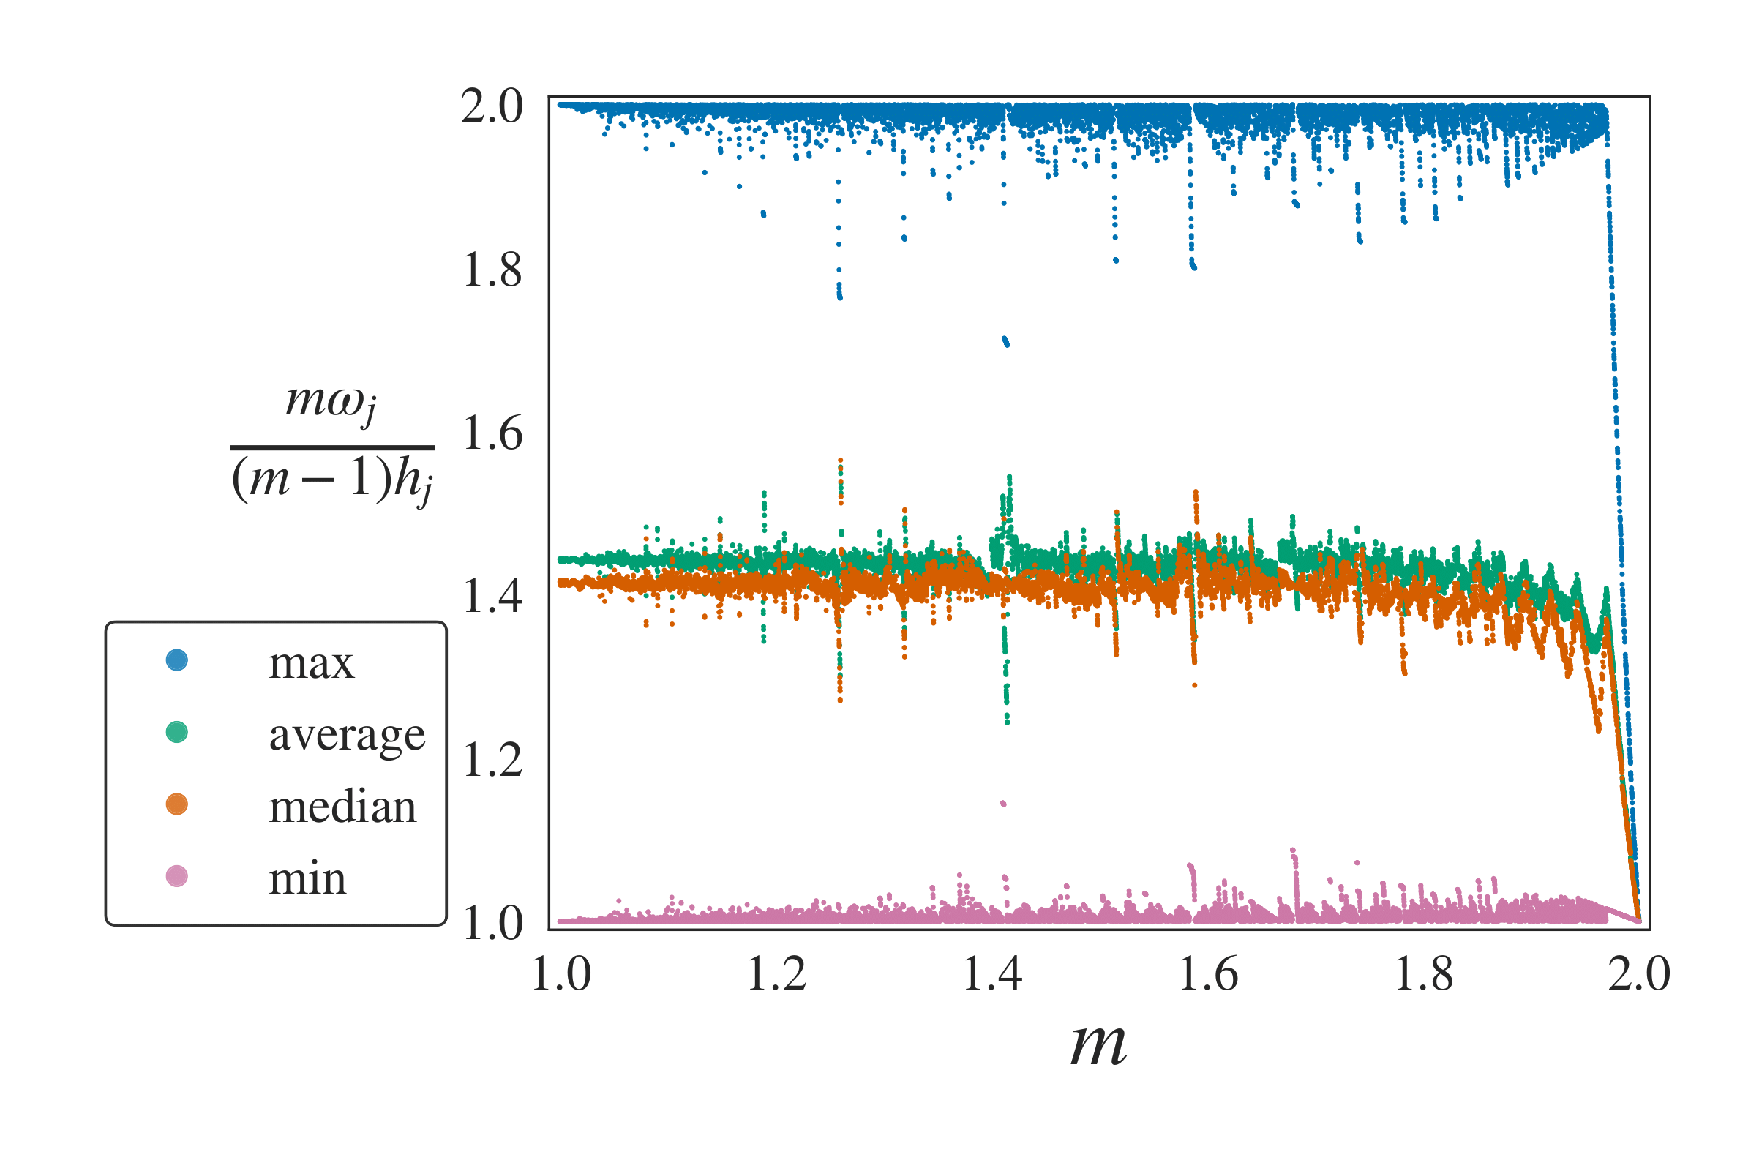
\includegraphics[clip, width= 0.99\textwidth]{2.1Rested/fig/delay_ratio.pdf}
\caption{Impact of $m$ on the minimum, maximum, average and median ratio among $\left\{\nicefrac{m \omega_j}{\pa{m-1}h_j}\right\}_j$.}
\label{fig:delay-ratio}
\end{figure*}

In Figure~\ref{fig:delay-ratio}, we display for each value of $m$ the maximum, minimum, median and average of the sequence $ \left\{ r_j\right\}_j$. Notice that $h_j = 10^{15}$ is much larger than the horizon usually considered in bandits experiments, even to characterize asymptotic performance \citep{chapelle2011empirical, kaufmann2012bayesian, lattimore2018refining}. Hence, the displayed minimum and maximum are valid empirical bounds for real application.

For more than $90\%$ of the values of $m$, the minimum is below $1.02$, the maximum is larger than $1.95$, and the median and mean are between $1.35$ and $1.45$. It shows that our theory is tight in general to characterize the best and worst possible normalized period. 

There are deviations to this general case. First, when $m\rightarrow 2$, the ratio tends to $1$ for all $j$. This is indeed the value when $m=2$. When we compare $m=1.9$ and $m=2$ on Figures~\ref{fig:delay-int} and~\ref{fig:delay-general}, we see that the normalized delay is drifting for $m=1.9$: the updates are synchronous and the normalized delay is $\sim 50 \%$ for the first statistics, but it becomes larger when $j$ is increasing. We conjecture that the closer $m$ is to 2, the slower is the drift.

Second, there are also local deviations (e.g near $m \sim 1.42$). They correspond to values of $m$ such that $m^{k}$ (with $k$ a small integer) is a power of two. In that case, the ratios $\left\{r_j\right\}_j$ are cycling in the regime $h_j >> 1$ (\ie when the rounding effect is negligible and $h_{j+1} \sim m\cdot h_j$)  and take only $k$ values up to small rounding perturbations. These values can either be quite good or quite bad. In fact, due to the rounding, these values are slowly drifting. We can try to control the drift by increasing or decreasing $m$ very slightly to improve the median or the average delay for a given horizon. 

As we can see on Figure~\ref{fig:delay-ratio}, it is very sensitive to the exact value of $m$. For instance, with $\epsilon = 1e^{-5}$,  $m = \pa{1-\epsilon} \times 2^{\nicefrac{1}{3}}$ has an average ratio of $1.29$ while $ m= \pa{1+\epsilon} \times 2^{\nicefrac{1}{3}}$ has an average ratio of $1.55$. Indeed, the normalized delay is not the same for a statistic which is updated just before the precedent one ($r_j \sim 1$) or for one which is updated just after ($r_j \sim 2$) . When the update of $\peff$ is just before, it is refreshed with almost $h_{j-1}$ samples, which is the best possible value. When it is just after, it is refreshed with $\sim h_{j-2}$ which is close to the worse one. Due to this discontinuity, it is hard to take advantage of these local deviation. %For the very long horizon $10^{15}$, we provide in Table~\ref{} interesting values of $m$ associated to local minima of the average of $\left\{r_j\right\}_j$. %TODO ?

To conclude, non-integer values for $m$ leads to a larger ratio $r_j$ than integer values (twice larger in the worst case, $\sim 1.4$ in average). However, the interesting quantity is the normalized period, which is equal to $\nicefrac{\pa{m-1}r_j}{m}$. For $m=2$, the normalized period is $50\%$ for all the statistics $j\geq1$. In order to achieve a lower value in the worst case, one should choose $m\leq \frac{4}{3}$. If we target a lower value in average, one should choose $m\leq 1.56$. It shows that non-integer values are especially interesting when $m\rightarrow 1$. Yet, there is no free lunch: the complexity of \EFFU scales with $\cO\pa{\log_m T}$ which diverges with $\nicefrac{1}{m-1}$ when $m\rightarrow 1$.



\subsubsection{Proofs}
\begin{proof}[Proof of Proposition~\ref{prop:effu-delay-int}]
When $m$ has an integer value, we have, 
\[
h_j = \ceil{m \cdot h_{j-1}} = m \cdot h_{j-1} = \dots = m^j\cdot h_0 = m^j.
\]
For $j=0$, $\hmu_{i,\,\tteff}^1$ is updated at every update at Line~\ref{algline:effu-update-first-hmu}. Hence, $\omega_0 =1$. 
For $j=1$, $h_1 =m$ is initialized after $m$ pulls. At this round, we set $n_i^{h_1}$ to the value in $n_i^{h_0}$ which is equal to $1$. Indeed, the first statistic is always up to date. Hence, the next update is after $m-1$ pulls. At this round, the pending statistics is again refreshed with $p_0$ which contains $1$ sample and, recursively, we can conclude that  $\hmu_{i,\,\tteff}^{h_1}$ is updated every $\omega_1 = m-1 =   \frac{m-1}{m} h_1$.

By induction, let $j$ such that the statistic $j-1$ is updated periodically every $\omega_{j-1} = \pa{m-1} m^{j-2}$ pulls from pull $m^{j-1}$. $\hmueff$ is initialized after $m^j$ pulls (Line~\ref{algline:effu-refresh-hmu}) . It is synchronized with the $m$-th update of statistic $\hmu_{i,\,\tteff}^{h_{j-1}}$. Indeed,
\[ m^j = m \cdot m^{j-1} =  m^{j-1} + m \omega_{j-1}.\]

Notice that we sort $\Him$ in the decreasing order at Line~\ref{algline:effu-refresh-start}, hence $\neff$ is updated with $n_i^{h_{j-1}} = m^{j-1}$ before it is itself refreshed with $n_i^{h_{j-2}}$  (Line~\ref{algline:effu-refresh-n}).  Hence, $\hmueff$ is updated for the first time after $\omega_j =h_{j} - \neff =  m^j - m^{j-1} = (m-1) m^{j-1} = m \omega_{j-1}$ pulls, \ie after $m^{j} + (m-1) m^{j-1}$ pulls of arm $i$. Again, this update is synchronized with the update of the lower order statistic:
\[ m^j +\omega_j =  m^{j} + (m-1) m^{j-1} =  m^{j-1} + 2m \omega_{j-1}.\]
Hence, the pending statistic $\peff$ is again refreshed with $n_i^{h_{j-1}} = m^{j-1}$ sample. Recursively, we can repeat the very same argument and show that $\hmueff$ is updated every $\omega_j = \pa{m-1} m^{j-1}$ pulls from pull $m^{j}$.
\end{proof}

\begin{proof}[Proof of Proposition~\ref{prop:effu-delay-periodic}]
We will prove this property by induction on $j$.  When $j=0$, the updates happen at every round. Hence, $\omega_0 =1$. Let $j$ such that $\hmu_{i,\,\tteff}^{h_{j-1}}$ is refreshed periodically with period $\omega_{j-1}$. $\hmueff$ is initialized after $h_j$ pulls. At that round $\peff$ is initialized with the current value of $p_i^{h_{j-1}}$ which contains $n_i^{h_{j-1}}$ samples. Since statistic $j-1$ is updated with period $\omega_{j-1}$, $n_i^{h_{j-1}}$  takes its value between $h_{j-1} -\omega_{j-1} +1$ and $h_{j-1}$. At pull $h_{j-1}$, it was initialized with value $h_{j-1} -\omega_{j-1} +1$. Then, it is increased by one at every pull and refresh at $h_{j-1} -\omega_{j-1} +1$ when it reaches value $h_j$. Therefore, at pull $h_j$, we have,
\begin{equation}
\label{eq:ni}
n_i^{h_{j-1}}\pa{h_j} = h_{j-1} -\omega_{j-1} +1 + \pa{h_j - h_{j-1} -1  \mod \omega_{j-1}}.
\end{equation}
with $n_i^{h_{j-1}}\pa{h}$, the value of $n_i^{h_{j-1}}$ at the end of the $h$-th pulls of arm $i$. The $-1$ is caused by the backward loop (Line~\ref{algline:effu-refresh-start}: when $h_j -h_{j-1} \mod \omega_{j-1}$, the updates are synchronized such that it minimizes the delay (like in the integer case). The next update of $\hmueff$ will happen in 
\begin{align*} 
\omega_j &\triangleq h_{j} - n_i^{h_{j-1}}\pa{h_j} \\
&= h_{j} - \pa{h_{j-1} -\omega_{j-1} +1 + \pa{h_j - h_{j-1} -1  \mod \omega_{j-1}}} 
\\&= \omega_{j-1} +h_j - h_{j-1} -1 -  \pa{h_j - h_{j-1} -1  \mod \omega_{j-1}} 
\\&=  \omega_{j-1}  \pa{1 + \floor{\frac{h_j - h_{j-1} -1}{\omega_{j-1}}}}
\end{align*}
The second line is justified by Equation~\ref{eq:ni}. The last line uses $a - a\mod b = b \floor{\nicefrac{a}{b}}$. Hence, the first delay $\omega_j$ is a multiple of $\omega_{j-1}$. Therefore, $n_i^{h_{j-1}}\pa{h_j + \omega_j} =n_i^{h_{j-1}}\pa{h_j}$ and $\hmueff$ is refreshed with the same number of sample than its initialization, and the delay until the second update is $h_j - n_i^{h_{j-1}}\pa{h_j + \omega_j} = n_i^{h_{j-1}}\pa{h_j}=\omega_j$. Recursively, we show that  $\hmueff$ is updated periodically with period $\omega_j$.
\end{proof}

\begin{proof}[Proof of Proposition~\ref{prop:effu-delay-m2}]
By \emph{reductio ad absurdum}, we consider the smallest $j\geq 1$ such that  $\omega_{j+1} > 2\cdot \omega_{j}$. A necessary and sufficient condition according to Proposition~\ref{prop:effu-delay-periodic} is that 
\begin{equation}
\label{eq:hj1}
h_{j+1} - h_j -1 \geq  2\omega_j. 
\end{equation}

When $1<m<2$, $h_0=1$, $\omega_0=1$ (as for any $m$), $h_1 = \ceil{m\cdot h_0}  = 2$,  and $\omega_1 = 1$ (according to Prop~\ref{prop:effu-delay-periodic}). Hence, $j \geq 1$.  Since $j\geq 1$ is the smallest value such that $\omega_{j+1} > 2\cdot \omega_{j}$, we have that either $\omega_j = \omega_{j-1}$ or $\omega_j = 2 \cdot \omega_{j-1}$. If $\omega_j = \omega_{j-1}$, we have according to Proposition~\ref{prop:effu-delay-periodic},
\[
h_j - h_{j-1} -1   < \omega_{j-1} = \omega_j. 
\]

If $\omega_j = 2 \cdot \omega_{j-1}$, we have with the same argument, 
\[
h_j - h_{j-1} -1   < 2\cdot \omega_{j-1} = \omega_j. 
\]

Since $h_j$, $h_{j-1}$ and $\omega_j$ are integers, we have 
\begin{equation}
\label{eq:hj2}
 h_j - h_{j-1} -1   < \omega_j \implies h_j - h_{j-1} \leq \omega_j.
 \end{equation}

Using $h_{j+1} = \ceil{m \cdot h_j}$,
\begin{equation}
\label{eq:hj3}
h_{j+1} - h_j -1  = \ceil{m \cdot h_j} - \ceil{m \cdot h_{j-1}} -1 \leq m \pa{h_j - h_{j-1}}
 \end{equation}
 
 Plugging Equations~\ref{eq:hj1}, \ref{eq:hj2} and~\ref{eq:hj3}, 
 \[ m \pa{h_j - h_{j-1}} \geq 2\pa{h_j - h_{j-1}}. \]

This is impossible for $m<2$ and $h_j > h_{j-1}$ (which is the case when $m>1$).  Hence, we conclude that there exists no integer $j$ such that $\omega_{j+1} > 2 \cdot \omega_j$.

\end{proof}

\begin{proof}[Proof of Proposition~\ref{prop:effu-delay-ub}]
We want to upper bound the ratio $\nicefrac{\omega_j}{h_j}$ for all $j$ such that $\omega_j>1$.  When $m < 2$ we have either $\omega_{j} = \omega_{j-1} $ or $\omega_{j} = 2 \cdot \omega_{j-1}$ (Prop.~\ref{prop:effu-delay-m2}). We first study the case where $\omega_{j} = 2 \cdot \omega_{j-1}$, \ie (Prop;~\ref{prop:effu-delay-periodic}),
\[
h_j - h_{j-1} - 1 \geq \omega_{j-1} = \nicefrac{\omega_{j}}{2}.
\]

Using $h_j = \ceil{m\cdot h_{j-1}}\implies h_{j-1} = \floor{\nicefrac{h_j}{m}}$, 
\[
h_j - h_{j-1} - 1 = h_j - \floor{\nicefrac{h_j}{m}} - 1  \leq \frac{m-1}{m} h_j.
\]

Plugging the two last equations leads to, 
\[
\frac{\omega_j}{h_j} \leq \frac{2 \pa{m-1}}{m}\cdot
\]


We notice that $\left\{h_j\right\}_{j \in \NN}$ is an increasing sequence. When $\omega_{j} = \omega_{j-1}$,  we have $\nicefrac{\omega_{j}}{h_j} < \nicefrac{\omega_{j-1}}{h_{j-1}}$. Therefore, for any $j$ such that $d_j > 1$ we can find the largest $j'\leq j$ such that $\omega_{j'} = 2 \cdot \omega_{j'-1}$ and compare, 
\[
\frac{\omega_j}{h_j} \leq \frac{\omega_j}{h_j'} = \frac{\omega_j'}{h_j'} \leq \frac{2 \pa{m-1}}{m}\cdot
\]
\end{proof}

\subsection{{\EFFFEWA} ($\piEF$) and {\EFFRAW} ($\piER$)}
{\EFFFEWA} ($\piEF$) and {\EFFRAW} ($\piER$) are the two efficient versions of our initial algorithms. With an hyperparameter $m>1$, they use \EFF instead of \UPDATE (Lines~\ref{algline:fewa-update1} and~\ref{algline:fewa-update2} in \FEWA and Lines~\ref{algline:raw-update1} and~\ref{algline:raw-update2} in \RUCB). Therefore, they use $\left\{\hmueff\right\}_{i,h_j\in \Him}$ instead of $\left\{\hmu_i^h\right\}_{i,h \leq \Nitmone}$. 

More precisely, in \FEWA, we replace the increment $h\gets h+1$ by $h\gets\ceil{m\cdot h}$ at Line~\ref{algline:fewa-window}. Hence, the next set is not called $\arms_{h+1}$ but $\arms_{\ceil{m\cdot h}}$ (Line~\ref{algline:fewa-filter} in \FEWA and Line~\ref{algline:filter-add} in \FILTER). Finally, at Lines~\ref{algline:fewa-condition} and~\ref{algline:fewa-pull}, the condition is not $N_{i_t}=h$ but $N_{i_t} \leq h$. In the \FILTER procedure, we also change $\hmu_i^h$ by $\hmu_{i,\,\tteff}^h$ at Lines~\ref{algline:filter-max} and~\ref{algline:filter-delta}. In \RUCB, we only change the $h\leq N_i$ by $h_j \in \Him$ and $\hmu_i^h$ by $\hmueff$ in the index computation at Line~\ref{algline:raw-pull}.

\begin{proposition}
At any round $t$, \EFFFEWA and \EFFRAW tuned with hyperparameter $m$ have a $\cO\pa{K\log_m\pa{t}}$ worst-case time and space complexity.
\end{proposition}
\begin{proof}
For each arm, the algorithms use the statistics created and maintained by \EFFU plus a handful of variables (such as $t$). Hence, the space complexity is the sum of the complexities of \EFFU (see Prop.~\ref{prop:effu-complexity}) for each arm, \ie

\[ 
\sum_{i \in \arms} \cO\pa{\log_m\pa{\NiT}}\leq \cO\pa{K\log_m\pa{T}}.
\] 

At every round $t$, the algorithms do one call of \EFFU, which costs at most $\cO\pa{\log t}$. For each of the $\cO\pa{K\log_m t}$, \EFFRAW computes one ucb with unit cost $\cO\pa{1}$. For each of the $K$ arms, we find the minimum ucb among the $\cO\pa{\log_m t}$ ones. It costs $\cO\pa{K\log_m t}$ in total. Finally, we select the arm with the largest index, which costs $\cO\pa{K}$. Hence, the worst-case time complexity at any round $t$ is $\cO\pa{K\log_m t}$.

\EFFFEWA uses the procedure \FILTER  at most for each existing window, \ie $\cO\pa{\log_m\pa{t}}$. The inner time complexity of \FILTER scales with $|\arms_h| \leq K$. Therefore, in the worst case, the time complexity of \EFFFEWA at any round $t$ is also bounded by $\cO\pa{K\log_m\pa{t}}$.
\end{proof}

\subsection{Regret analysis}
In our analysis, the particularities of \RAWUCB and \FEWA only appear in Proposition~\ref{prop:prb_favorable_event} and Corollary~\ref{cor:core-RAW-FEWA}. We will derive analogous results for \EFFRAW and \EFFFEWA when $m=2$. The upper-bounds will directly follow with no additional effort. We discuss the case $m\neq 2$ at the end of this Subsection. 
\paragraph{A favorable event for efficiently updated adaptive windows}
\begin{proposition}
\label{prop:prb_favorable_event_eff}
For any round $t$ and confidence $\delta_{t} \triangleq 2t^{-\alpha}$, let 
%
\begin{equation*}
\!\HPeff\! \triangleq\! \Big\{ \forall i\!\in\!\arms,\ \forall n \!\leq\! t\!-\!1 ,\ \forall h_j \in \Him(n), \big| \hmueff(t, \pi) - \bmueff(t,\pi) \big| \!\leq\! c(h_j, \delta_{t}) \!\Big\}
\end{equation*}
 be the event under which the estimates at a round $t$  are all accurate up to $c(h,\delta_{t}) \triangleq \sqrt{2 \subgaussian^2\log(2/\delta_t)/h}$. Then, for a policy $\pi$ which pulls each arms once at the beginning, and for all $t>K$,
\[
\PPempty\Big[\bar{\HPtwo}\Big] \leq 3Kt\delta_t= 6Kt^{1-\alpha}\,\cdot
\]
\end{proposition} 
\begin{remark}
The probability of the unfavorable event $\bar{\HPtwo}$ scales with $\cO\pa{t^{1-\alpha}}$ compared to $\cO\pa{t^{2-\alpha}}$ for $\bar{\HPevent}$ because the efficient algorithms construct less statistics. It means that our theory will hold for a wider range of $\alpha$. Yet, this benefits is only theoretical. The union bound in Proposition~\ref{prop:prb_favorable_event} is not tight because the different events share the same data. In practice, it leads to conservative tuning of the confidence bounds and one can decrease $\alpha$ to get better performance. 
\end{remark}

\begin{proof}
As in Propositions~\ref{prop:prb_favorable_event_SWA} and~\ref{prop:prb_favorable_event}, we have to count the number of statistics that are required to hold in the confidence region. 
We call  $u_j(n)$ the number of different values taken by variable $\hmueff$ after $t$. According to Proposition~\ref{prop:effu-delay-int}, $u_0(n) = n \leq t $ because statistic $0$ is created at the first round and updated at every round ($\omega_0=1$). For $m=2$ and $j\geq 1$,  $\hmueff$ is created after $h_j= 2^j$ pulls and then updated every $\omega_j = 2^{j-1}$. Hence, 
\[
\forall j \geq 1 \text{ and } h_j \leq n, u_j(n) = 1 + \floor{\frac{n-h_j}{\omega_j}} \leq \frac{n}{2^{j-1}} - 1 \leq \frac{n}{2^{j-1}}\cdot
\]

We do the union bound, 
\begin{align*}
    \PPempty\Big[\bar{\HPtwo}\Big] &\leq \sum_{i \in \arms} \sum_{j=0}^{|\Him(\Nit)|} u_j(t) \delta_t \\
    &\leq \sum_{i \in \arms} \pa{t  + \sum_{j=1}^{|\Him(\Nit)|} \frac{t}{2^{j-1}}} \delta_t \\
    &\leq 3Kt\delta_t.
\end{align*}
\end{proof}

\begin{lemma}
\label{lem:core-eff}
At any round $t$ on favorable event $\HPtwo$, if arm~$i_{t}$ is selected by $\pi \in \left\{\piEF, \piER\right\}$ tuned with $m=2$, for any $h \leq \Nitmone$,  the average of its $h$ last pulls cannot deviate significantly from the best available arm at that round, i.e.,
\begin{equation*}
\bmu^{h}_{i_t}(t-1,\pi) \geq \max_{i \in \arms} \mu_{i}(t,\Nitmone)- \frac{C_\pi}{\sqrt{2\alpha}} c(h, \delta_t) \quad \text{with } 
\begin{cases}
C_{\piER} = \frac{4\sqrt{\alpha}}{\sqrt{2}-1}\\
C_{\piEF} = \frac{8\sqrt{\alpha}}{\sqrt{2}-1}
\end{cases}\cdot
\end{equation*}
\end{lemma}

\begin{proof}
Like for Lemma~\ref{lem:core-FEWA} (see its proof), our proof is done in a more general rotting framework that can be used in the next chapter. We denote by $\bar{\mu}^{hh'}_i(t-1,\pi)$ and $\hat{\mu}^{hh'}_i(t-1,\pi)$ the true mean and empirical average associated to the $h'-h$ samples between the $h$-th last one (included) and the $h'$-th last one (excluded). Let $j_h \in \NN^\star$ such that:
$2^{j_h} -1 \leq  h < 2^{j_h+1}$.
\begin{equation}
\label{eq:eff-decompo}
\bar{\mu}^{h}_{i_t}(t-1,\pi) \geq \bar{\mu}^{2^{j_h}-1}_{i_t}(t, \pi) = \sum_{j=0}^{j_h-1} \frac{2^j}{2^{j_h}-1} \bar{\mu}^{2^{j}2^{j+1}}_{i_t}(t, \pi).
\end{equation}
The inequality follows because the reward is decreasing and $h\geq 2^{j_h}-1$. Then, we decompose the average in a weighted sum of averages of geometrically expanding windows. Since the reward is decreasing we have that,
\begin{equation*}
\forall k \leq 2^j, \quad \bar{\mu}^{2^{j}2^{j+1}}_{i_t}(t, \pi) \geq \bar{\mu}^{k : k+2^{j}}_{i_t}(t, \pi).
\end{equation*}

$\hmuiteff$ contains $2^j$ samples among the $2^{j+1}-1$ last ones (see Proposition~\ref{prop:effu}). Setting $k\leq 2^j$ to the current delay of the statistics $\hmuiteff$ (see Point~\ref{list:effu-delay} in Proposition~\ref{prop:effu}), we can write,

\begin{equation}
\label{eq:hmueff-link}
\bar{\mu}^{2^{j}2^{j+1}}_{i_t}(t, \pi) \geq \bar{\mu}^{k : k+2^{j}}_{i_t}(t, \pi) = \bmuiteff\geq  \hmuiteff - c(2^j, \delta_t),
\end{equation}
where we use that we are on $\HPtwo$ for the last inequality. Therefore, gathering Equations~\ref{eq:eff-decompo} and~\ref{eq:hmueff-link}, 
\begin{equation}
\label{eq:eff-general}
\bar{\mu}^{h}_{i_t}(t, \pi) \geq \sum_{j=0}^{j_h-1} \frac{2^j}{2^{j_h}-1} \pa{\hmuiteff - c(2^j, \delta_t)}.
\end{equation}
Now, we will use the mechanics of the two algorithms. On the first hand, for $\EFFRAW$, we make the index appear in the inequality,
\begin{align}
 \bar{\mu}^{h}_{i_t}(t, \piER) &\geq \sum_{j=0}^{j_h-1} \frac{2^j}{2^{j_h}-1} \pa{\hmuiteff - c(2^j, \delta_t)} \nonumber\\
 &=\sum_{j=0}^{j_h-1} \frac{2^j}{2^{j_h}-1} \pa{\hmuiteff + c(2^j, \delta_t) - 2c(2^j, \delta_t)}\nonumber\\
 &\geq \min_{j \in H_{i_t, 2}} \pa{\hmuiteff + c(2^j, \delta_t)} - 2 \sum_{j=0}^{j_h-1} \frac{2^{j}}{2^{j_h}-1} c(2^j, \delta_t).
 \label{eq:effraw-index-appear}
 \end{align}
 %
 Then, we can relate the left part of the sum to the best current value $\mu_{\ist}(t,\Nisttmone)$,
 \begin{equation}
 \min_{j \in H_{i_t, 2}}  \pa{\hmuiteff + c(2^j, \delta_t)} \geq \min_{j \in H_{\ist,2}} \pa{\hmu_{\ist,\, \tteff}^{h_j} + c(2^j, \delta_t)}\geq  \bmu_{\ist,\, \tteff}^{h_{\min}} \geq \mu_{\ist}(t,\Nisttmone).
 \label{eq:effraw-index-use}
 \end{equation}
%
where $h_{\min} \in \argmin_{h_j \in H_{\ist,2}} \pa{\hmu^{h_j}_{\ist,\, \tteff} + c(h_j, \delta_t)}$.The first inequality follows because \EFFRAW selects the arm $i_t$ with the largest index. In particular, the index of $i_t$ is larger or equal to the index of $i^\star_t \in \argmax_{i\in \arms} \mu_i(t, N_{\ist,\,t})$. The second inequality holds on $\HPtwo$. The third inequality uses the decreasing of the reward. Putting Equations~\ref{eq:effraw-index-appear} and~\ref{eq:effraw-index-use}, we get,
\begin{equation}
\label{eq:effraw-result}
\bmu^{h}_{i_t}(t, \piER) \geq \mu_{\ist}(t,\Nisttmone)- 2 \sum_{j=0}^{j_h-1} \frac{2^{j}}{2^{j_h}-1} c(2^j, \delta_t).
\end{equation}
%
On the other hand, for \EFFFEWA, we know that the selected arm passes any filter of window $2^j \in H_{i_t, 2}$. Therefore, with $i_{\max} \in \argmax_{i \in \arms_{h_j}} \bmueff$, we can write,
\begin{flalign}
\qquad\hmuiteff &\geq \max_{i\in \arms_{h_j}} \hmueff -2c\pa{h_j, \delta_t} \nonumber && \text{Filtering rule}\\
\qquad&\geq \hmu_{i_{\max}, \, \tteff}^{h_j}  -2c\pa{h_j, \delta_t} \nonumber  && i_{\max} \in \arms_{h_j} \\
\qquad&\geq \bmu_{i_{\max}, \, \tteff}^{h_j} - 3c(h_j, \delta_t)\nonumber && \text{ on }\HPtwo \\
\qquad& = \max_{i\in \arms_{h_j}}  \bmueff -3c\pa{h_j, \delta_t}.
\label{eq:efffewa-3c}
\end{flalign}
%
We relate $\bmueff$ to the largest available value at the round $t$,
\begin{equation}
\label{eq:efffewa-ist-relation}
\max_{i\in \arms_{h_j}} \bmueff \geq \max_{i\in \arms_{1}}\bmu_{i,\tteff}^1 =  \max_{i\in \arms}\bmu_{i,\tteff}^1 \geq \bmu_{\ist,\tteff}^1 \geq  \mu_{\ist}(t, \Nisttmone).
\end{equation}
%
The last inequality follows from the decreasing of the reward and the before last from the definition of the maximum operator. The first one uses a similar argument than in Lemma~\ref{lem:core-FEWA}: $\max_{i\in \arms_{h_j}} \bmueff$ increases with $h_j$.  Indeed, on $\HPtwo$, 
\[  i_j \in \argmax_{i\in \arms_{h_j}} \bmueff \subset \arms_{h_{j+1}},\]
 because it cannot be at more than two confidence bounds from the best empirical value during the filter $h_j$. Thus, we get, 
\[
\max_{i\in \arms_{h_j}} \bmueff = \bmu_{i_j,\tteff}^{h_j} \leq \bmu_{i_j,\tteff}^{h_{j+1}} \leq \max_{i\in \arms_{h_{j+1}}}\bmu_{i,\tteff}^{h_{j+1}}. 
\]
The first inequality follows because $\bmu_{i_j,\tteff}^{h_{j+1}}$ contains reward sample which are either in $\bmu_{i_j,\tteff}^{h_j}$ or are older than the ones in $\bmu_{i_j,\tteff}^{h_j}$. Indeed, when $m=2$, $\hmu_{i, \, \tteff}^{h_{j+1}}$ is updated synchronously with $\hmueff$ (see Figure~\ref{fig:delay-int} and its section on delay). Hence, at each update of $\hmu_{i, \, \tteff}^{h_{j+1}}$, it contains all the samples of $\hmueff$ and the $2^j$ precedent ones. Thus, because the reward is decreasing, we have $\bmu_{i_j,\tteff}^{h_{j+1}} \geq \bmu_{i_j,\tteff}^{h_{j}} $.  The second inequality uses that $i_j \in \arms_{h_{j+1}}$. Gathering Equations~\ref{eq:eff-general}, \ref{eq:efffewa-3c} and~\ref{eq:efffewa-ist-relation}, we get 
%
\begin{equation}
\label{eq:efffewa-result}
\bmu^{h}_{i_t}(t, \piEF) \geq  \mu_{\ist}(t,\Nisttmone)- 4 \sum_{j=0}^{j_h-1} \frac{2^{j}}{2^{j_h}-1} c(2^j, \delta_t).
\end{equation}
%
With few lines of algebra, we reduce the sum,
\begin{flalign*}
\sum_{j=0}^{j_h-1} \frac{2^{j}}{2^{j_h}-1} c(2^j, \delta_t) &= \sum_{j=0}^{j_h-1} \frac{\sqrt{2}^{j}}{2^{j_h}\!-\!1} c(1, \delta_t) && c(2^j, \delta_t) = \frac{c(1,\delta_t)}{\sqrt{2^j}} \\
& = \frac{\sqrt{2}^{j_h} -1 }{\pa{\sqrt{2}-1}\pa{2^{j_h}-1}}c(1, \delta_t) && \sum_{n=0}^N q^n = \frac{q^{N+1}-1}{q-1}\\
& = \frac{1}{\pa{\sqrt{2}-1}\pa{\sqrt{2}^{j_h}+1}} c(1, \delta_t) && a^2\!-\!1 \!=\!  \pa{a\!-\!1}\!\pa{a\!+\!1}\\
& \leq  \frac{\sqrt{2}}{\pa{\sqrt{2}-1}\sqrt{2^{j_h+1}}} c(1, \delta_t) &&\sqrt{2^{j_h}} +1 \geq  \frac{\sqrt{2^{j_h+1}} }{\sqrt{2}} \\
& \leq \frac{\sqrt{2}}{\pa{\sqrt{2}-1}\sqrt{h}} c(1, \delta_t) &&  h \leq 2^{j_h+1}  \\
& = \frac{\sqrt{2}}{\sqrt{2}-1} c(h, \delta_t). &&  \frac{c(1,\delta_t)}{\sqrt{h}} = c(h, \delta_t)
%& \leq \frac{\sqrt{2}}{\sqrt{2}-1} c(h, \delta_t). && }  c(\cdot, \delta) \searrow
\end{flalign*}
%
Plugging this last equation in Equations~\ref{eq:effraw-result} and~\ref{eq:efffewa-result} leads to the final result,
\[
\bmu^{h}_{i_t}(t, \pi) \geq \max_{i \in \arms} \mu_{i}(t,\Nitmone)- \frac{C_\pi}{\sqrt{2\alpha}} c(h, \delta_t) \quad \text{with } 
\begin{cases}
C_{\piER} = \frac{4\sqrt{\alpha}}{\sqrt{2}-1}\\
C_{\piEF} = \frac{8\sqrt{\alpha}}{\sqrt{2}-1}
\end{cases}\cdot
\]
\end{proof}
Using Proposition~\ref{prop:prb_favorable_event_eff} and Lemma~\ref{lem:core-eff} instead of Prop.~\ref{prop:prb_favorable_event} and Corollary~\ref{cor:core-RAW-FEWA}, we can obtain similar problem dependent and independent bounds than for \FEWA and \RUCB. The proof directly follows from the precedent analysis. 
\begin{theorem}
\label{th:rested-PI-eff}
For any rotting bandit scenario with means $\{\mu_i\}_{i} \in \rewardSet^K$ and any time horizon $T$, $\pi \in \left\{\piER, \piEF \right\}$ run with $\alpha \geq 4$ and $m=2$ suffers an expected regret of
\begin{equation*}
\mathbb{E}[\regret(\pi)] \leq C_\pi\sigma \sqrt{\log\pa{T}}\pa{\sqrt{KT} +K} + 6KL \;\; \text{with } 
\begin{cases}
C_{\piER} = \frac{4\sqrt{\alpha}}{\sqrt{2}-1}\\
C_{\piEF} = \frac{8\sqrt{\alpha}}{\sqrt{2}-1}
\end{cases}\cdot
\end{equation*}
\end{theorem}
\begin{theorem}\label{th:rested-PD-eff}
For any rotting bandit scenario with means $\{\mu_i\}_{i} \in \rewardSet^K$ and any time horizon $T$, $\pi \in \left\{\piER, \piEF \right\}$ run with $\alpha \geq 4$ and $m=2$ suffers an expected regret of
\begin{align*}
\mathbb{E}\left[R_T(\pi)\right]  \leq \sum_{i\in \arms} \pa{\frac{C_\pi^2\sigma^2\log\pa{T}}{\Delta_{i,\hiT^+-1}} +  C_\pi\sigma\sqrt{\log\pa{T}} +6L } \\
\text{with } 
\begin{cases}
C_{\piER} = \frac{4\sqrt{\alpha}}{\sqrt{2}-1}\\
C_{\piEF} = \frac{8\sqrt{\alpha}}{\sqrt{2}-1}\\
\text{$\Delta_{i,h}$ and $\hiT^+$ defined in Equation~\ref{eq:hit+}.}
\end{cases}
\end{align*}
\end{theorem}
Among the differences, we notice that our theory holds for a larger range of $\alpha \geq 4$ but the constant $C_\pi$ is $\frac{\sqrt{2}}{\sqrt{2}-1} \sim 3.4$ times larger than their original counter part. We will show empirically in the next Subsection that it is mostly a theoretical artifact due to the more complex analysis. For instance, to derive Lemma~\ref{lem:core-eff}, we consider for simplicity that the statistics could be delayed up to $100\%$ their window size while we show in Proposition~\ref{prop:effu-delay-int} that the normalized period is at most $50\%$.

\begin{remark}
\textbf{Can we adapt our theory for {$m\neq2$}?} The case $m=2$ is less technical. First, $2$ is an integer, which avoids the messier analysis due to the ceil operator in $h_{j+1} = \ceil{m\cdot h_j}$. Moreover, in the proof of \EFFFEWA (Equation~\ref{eq:efffewa-ist-relation}), we use the strong synchronicity in the update which is the case when $m$ is an integer. Last the decomposition of $\hmu_{i}^h$ (Equations~\ref{eq:eff-decompo} to ~\ref{eq:eff-general}) is simpler on the geometric grid of parameter $2$. Yet, we believe that the proof could be adapted without major difficulties at least for \EFFRAW when $m<2$ (which is the most interesting case). 
\end{remark}

\subsection{Experimental Results}
\label{ss:eff-exp}
\subsubsection{Simulated efficient benchmark}
\paragraph{Setup.} We study a two-arm rotting bandit similar to the one presented in Subsection~\ref{subsec:rested-experiment1} but with a longer horizon $T = 10^6$. Like in the previous setups, the noise is Gaussian. There are one constant arm with value $0$ and one rotting arm which switches from $0.1$ to $-0.1$ after $\nicefrac{T}{4}$ pulls.

\paragraph{Algorithms.} In Figure~\ref{fig:rested-eff}, we compare the performance of \RAWUCB with \EFFRAW for different values of $m$. We use the value $\alpha = 1.4$ which is the best empirical value we found in the previous setups. We also display the best of the 3 versions of \wSWA that we already studied. We add the running time in Table~\ref{tab:time-figeff}. 
\begin{figure*}[h!]
\centering
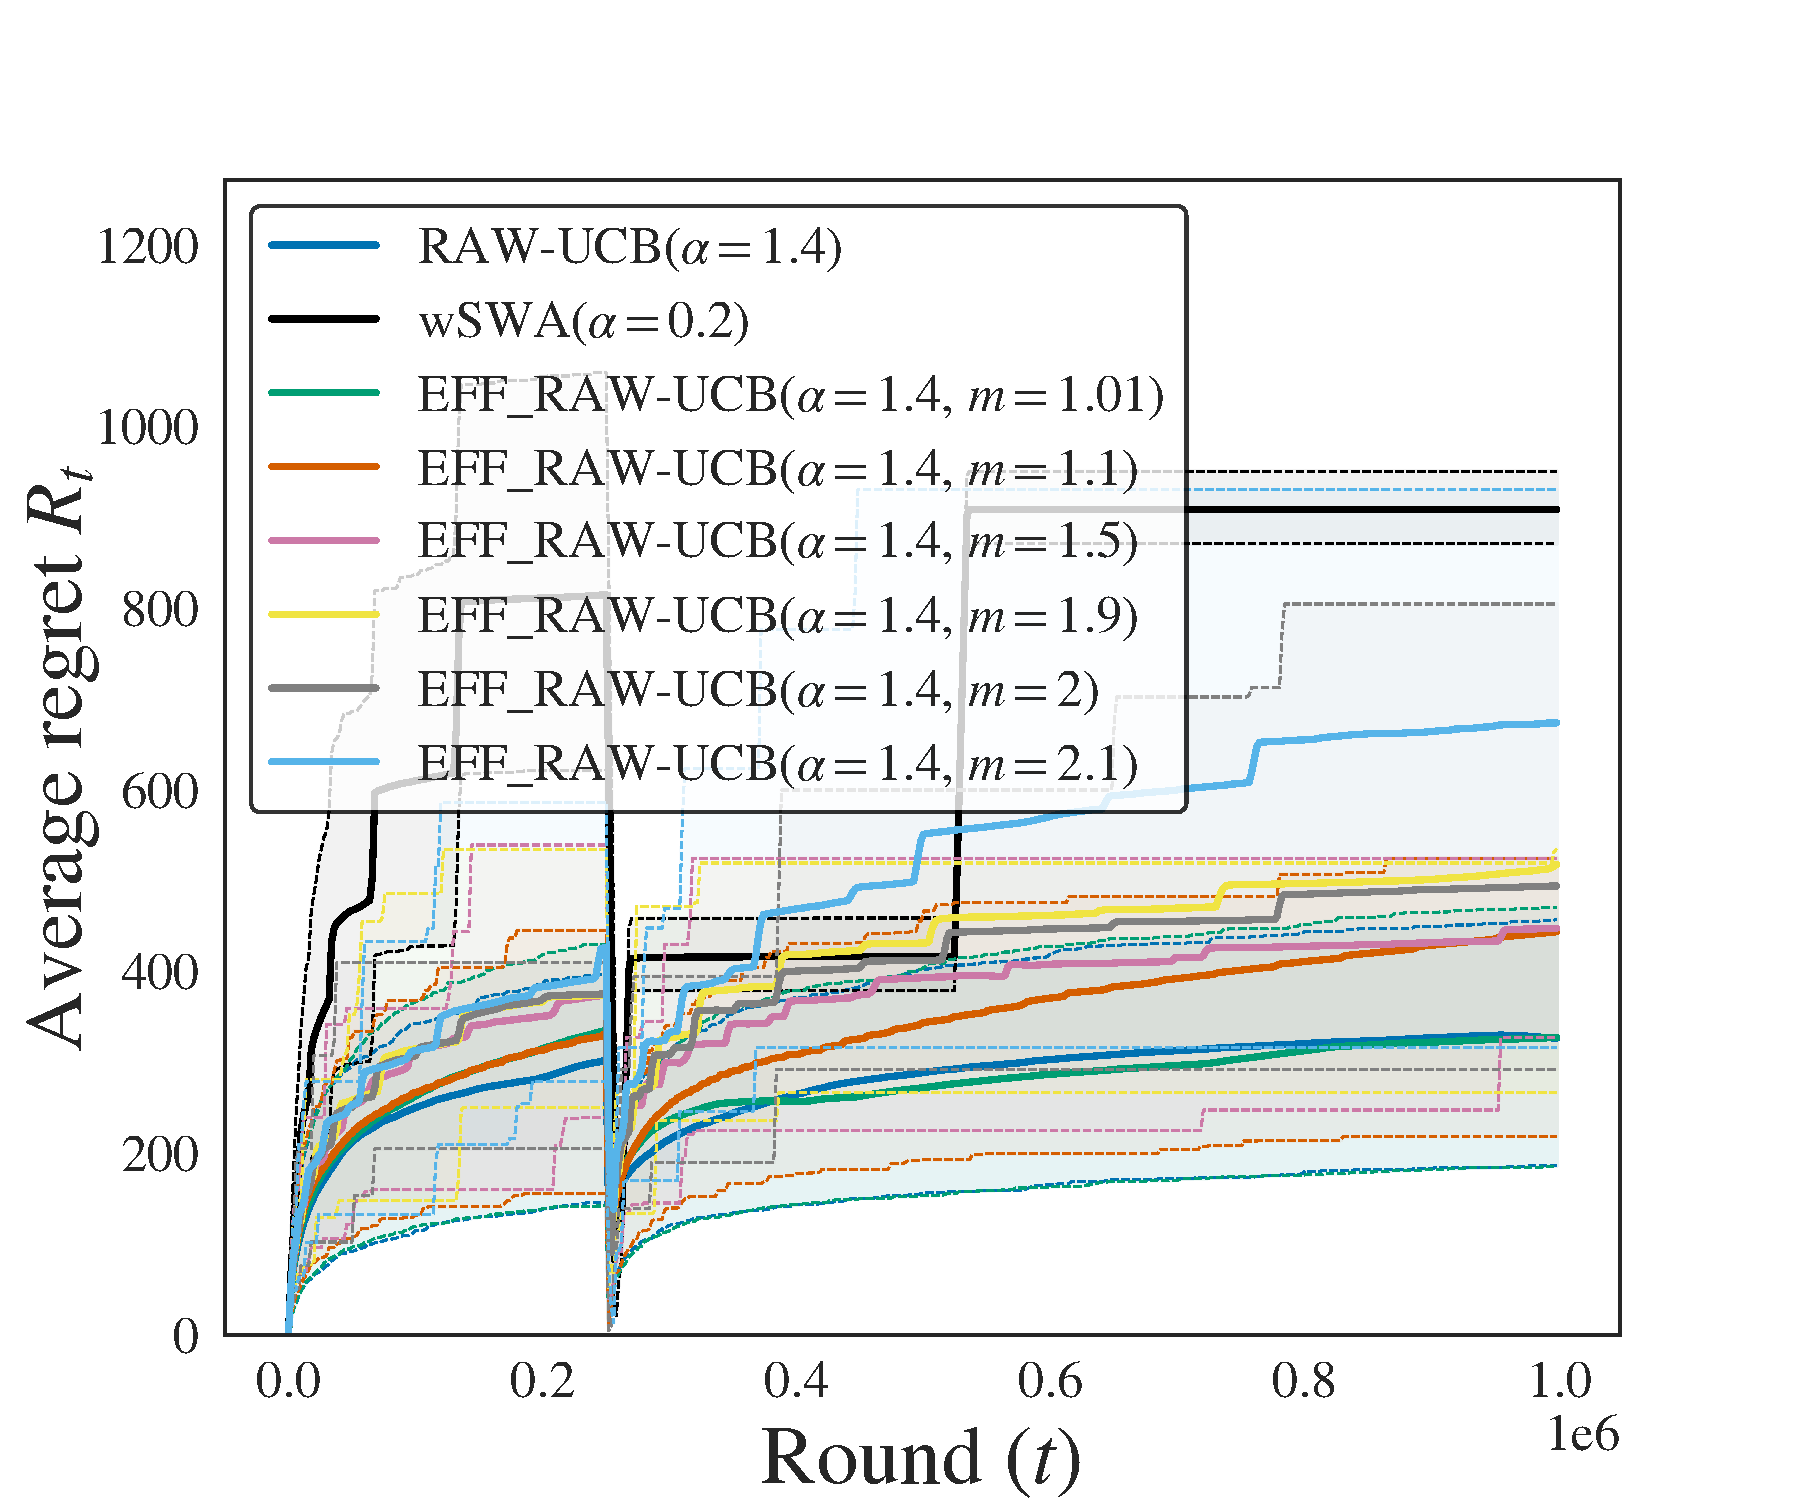
\includegraphics[width = 0.8\textwidth]{2.1Rested/fig/fig_eff.pdf}
\caption{Regret across time. Average over 1000 runs. We highlight the $\left[10\%, 90\%\right]$ confidence region.} 
\label{fig:rested-eff}
\end{figure*}

\begin{table}[ht!]
\centering
\begin{tabular}{|c|c|c|}
\hline
\textbf{Policy} &\textbf{Running time (s)} & \textbf{comparison w/ \RAWUCB}\\ \hline
\RAWUCB ($\alpha = 1.4$) & 38837      & 100$\%$                \\ \hline
\EFFRAW($\alpha = 1.4$, $m=1.01$)    & 169       & 0.4 $\%$             \\ 
\EFFRAW($\alpha = 1.4$, $m=1.1$)    & 121    & 0.3 $\%$                   \\ 
\EFFRAW($\alpha = 1.4$, $m=1.5$)    & 115    & 0.3 $\%$                  \\ 
\EFFRAW($\alpha = 1.4$, $m=1.9$)    & 112       & 0.3 $\%$               \\ 
\EFFRAW($\alpha = 1.4$, $m=2$)    & 119       & 0.3 $\%$               \\ 
\EFFRAW($\alpha = 1.4$, $m=2.1$)    &  114      & 0.3 $\%$               \\ \hline
\wSWA($\alpha = 0.002$)   & 41   & 0.1 $\%$                     \\ 
\wSWA($\alpha = 0.02$)    & 43  & 0.1 $\%$                      \\ 
\wSWA($\alpha = 0.2$)    & 49    & 0.1 $\%$                    \\ \hline
\end{tabular}
  \caption{Average running time and comparison with {\RAWUCB} for the efficient benchmark.}
  \label{tab:time-figeff}
\end{table}

\paragraph{Results.} Overall, the regret performance of \EFFRAW is up to $50\%$ worse than the performance of \RAWUCB. The worst versions correspond to larger values of $m$. Yet, there are few counter-examples: $m=2$ performs similarly to $m=1.9$ and $m=1.1$ performs similarly than $m=1.5$ at the end of the game. We remark that there are discontinuities in the regret of the efficient algorithms. It is because the statistics are not updated at every round. Hence, when one statistic is updated, it can change the behavior of the algorithm for many rounds. 

In terms of running time, the efficient trick drastically reduces the running time of \EFFRAW. While the theory suggests that there is no free lunch, we remark that setting a value very close to $1$ does reduce the running time and recover very similar regret performance. Surprisingly, the running time are quite similar for $m \in \bra{1.1, 2.1}$. The running time when $m=1.01$ is only 48 seconds (+ 40$\%$) larger than for $m=1.1$ while there are 10 times more confidence intervals to compute. Hence, we believe that the UCBs computation time for $m \in \bra{1.1, 2.1}$ is quite small compared to other fixed costs in the implementation (the reward generation, the $\log\pa{t}$ computation, etc.).   However, \wSWA is still faster than \EFFRAW. It is surprising because its complexity is $\cO\pa{T^{\nicefrac{2}{3}}}$, which is much larger than \EFFRAW 's $\cO\pa{K\log_m{T}}$. Yet, in practice, \wSWA computes $T^{\nicefrac{2}{3}}$ sums while \EFFRAW computes $\cO\pa{K\log_m{T}}$ ucb indexes (with a $\sqrt{\cdot}$ and a $\log$ function).

We believe that we could speed up \EFFRAW with low-level implementation tricks. For instance, the profiling of the code indicates that the $\log$ function is very expensive. One could compute faster the $\log(t+1)$ from the previous value $\log(t)$. Yet, these low-level implementation tricks are not in the scope of this thesis. 

\subsubsection{Simulated benchmark $\#$1 (2 arms) and $\#$2 (10 arms).}
\paragraph{Setup and Algorithms.} We study the two benchmarks described in Subsection~\ref{subsec:rested-experiment1} and Section~\ref{sec:rested-experiment}. In Figures~\ref{fig:rested-eff1} and~\ref{fig:rested-eff2}, we compare \RAWUCB with \EFFRAW for two values of m $\ev{1.1, 2}$.

\paragraph{Results.} For the two values, we remark that \EFFRAW have a slightly worse performance than \RAWUCB (up to $50\%$ for $m=2$). It confirms our theoretical analysis which suggests that the performance of \EFFRAW is only at a constant factor of the performance of \RAWUCB. It also confirms that the smaller the $m$, the less regret we suffer. 
\begin{figure*}[!ht]
\centering
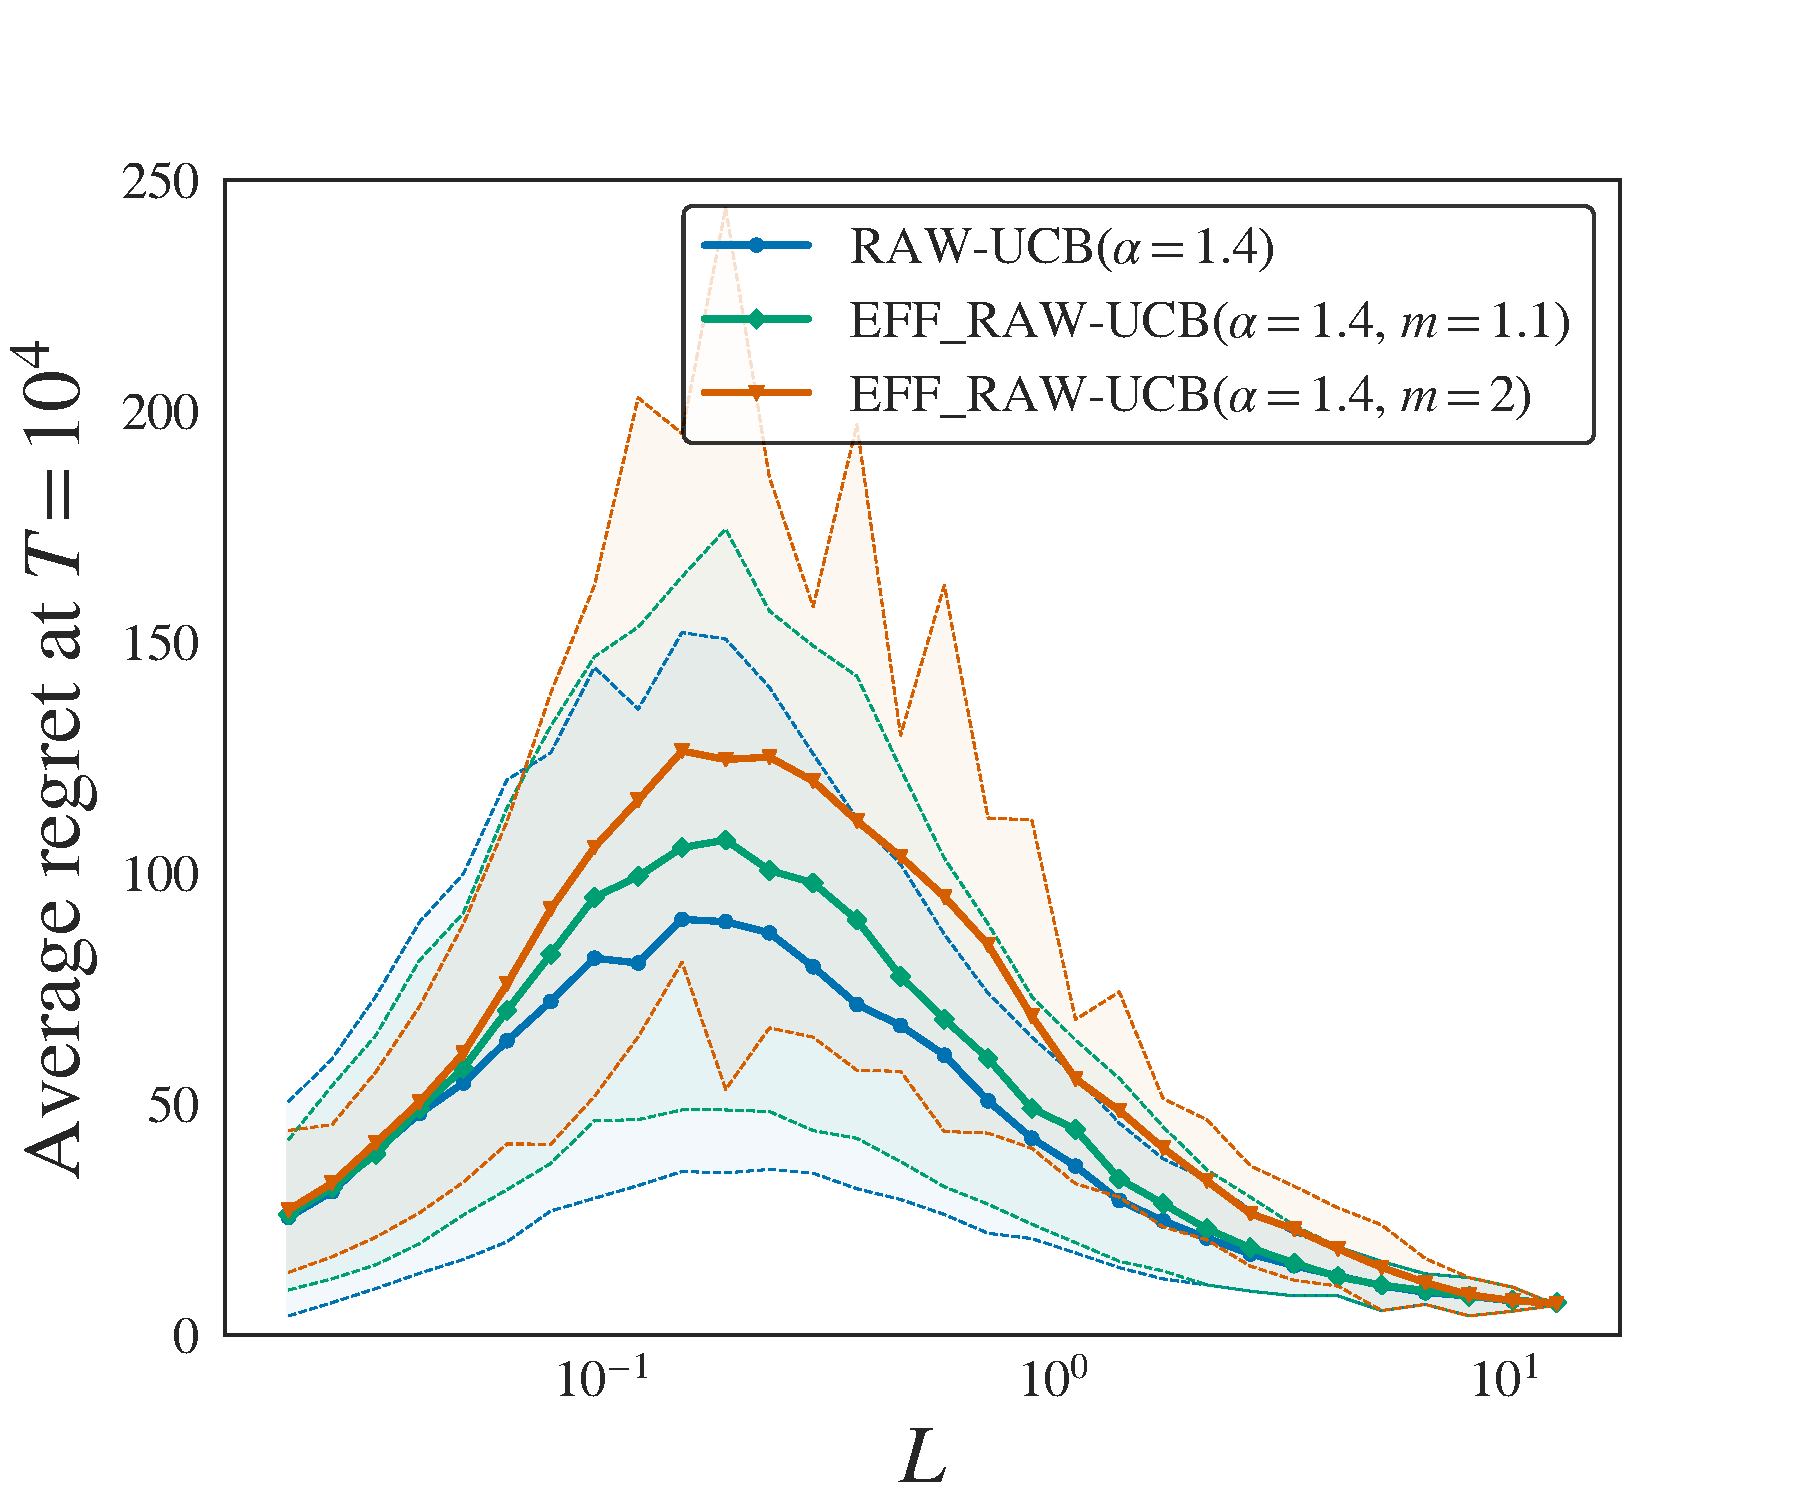
\includegraphics[clip, width= 0.51\textwidth]{2.1Rested/fig/fig1A_eff.pdf}
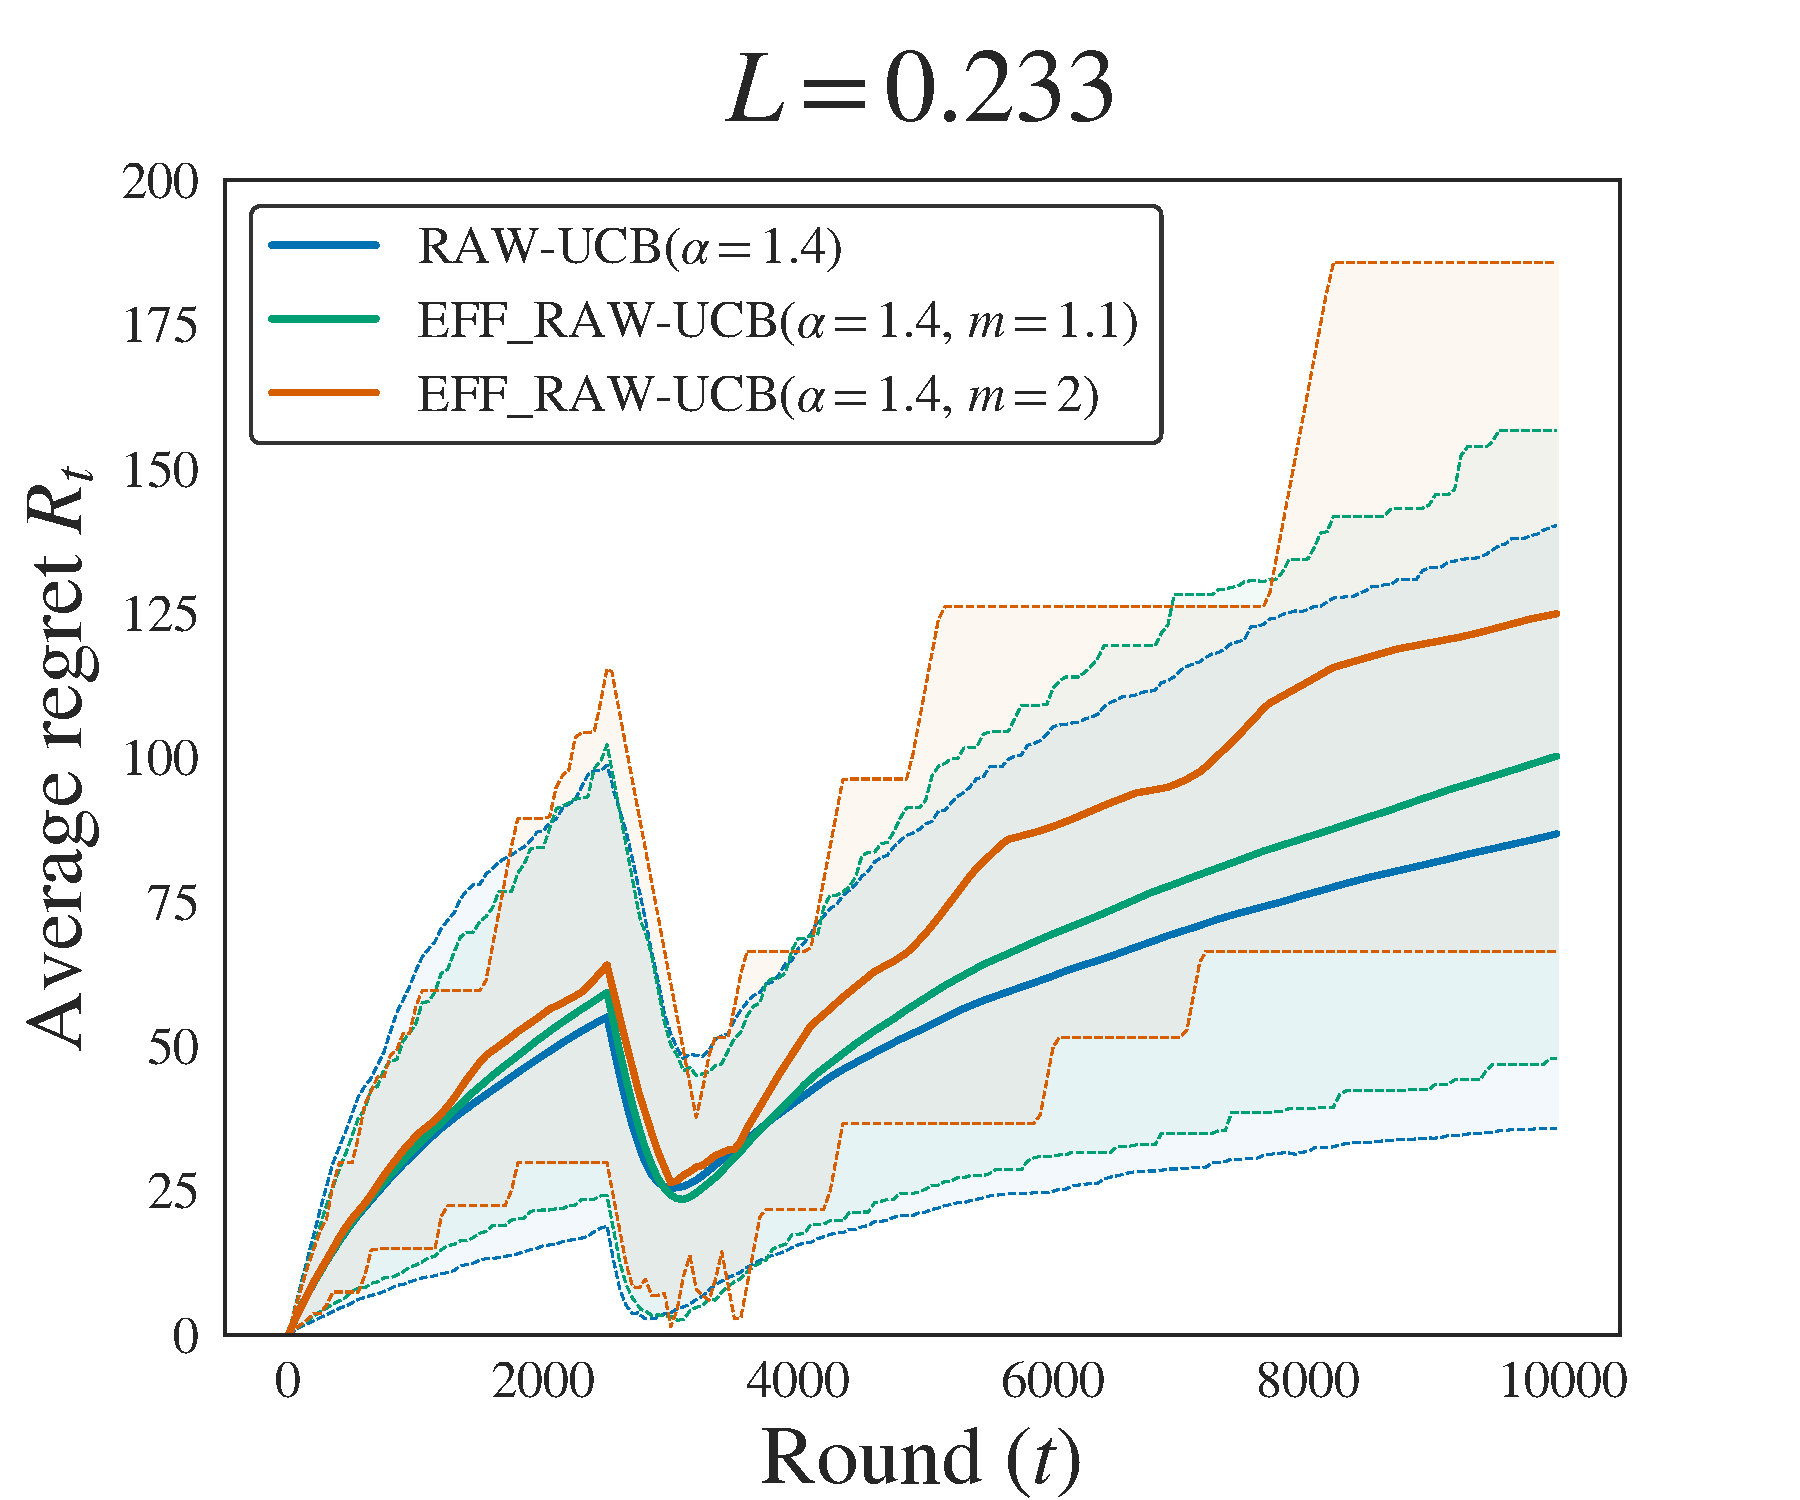
\includegraphics[clip, width= 0.49\textwidth]{2.1Rested/fig/fig1B_eff.pdf}
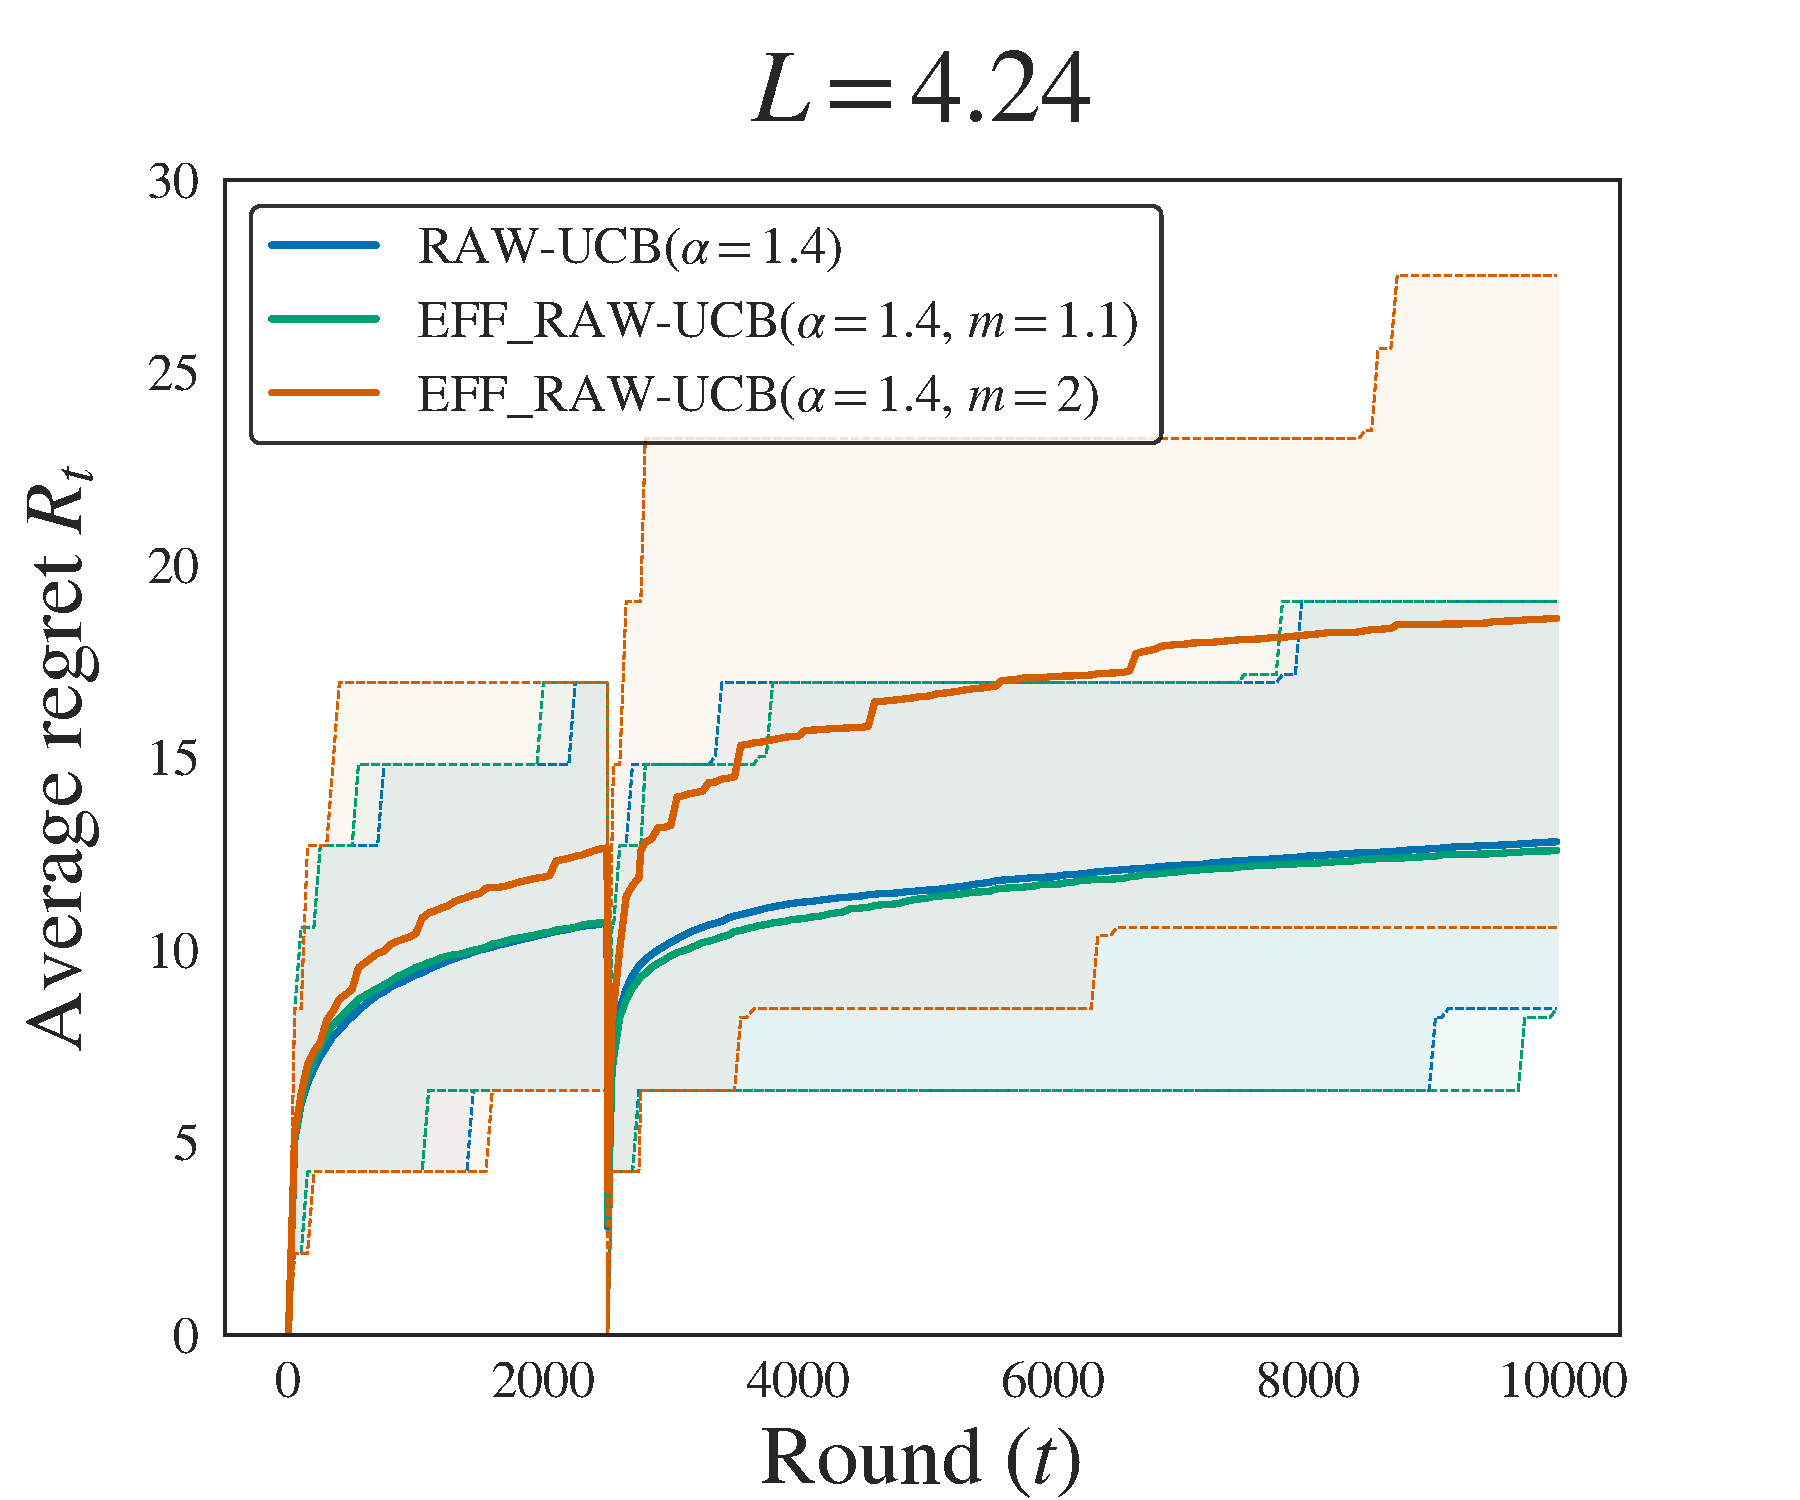
\includegraphics[clip, width= 0.49\textwidth]{2.1Rested/fig/fig1C_eff.pdf}
\caption{\textbf{Top:} Regret at the end of the game for different values of $L$. \textbf{Bottom:} Regret across time for two values of $L$. Average over 1000 runs. We highlight the $\left[10\%, 90\%\right]$ confidence region.}
\label{fig:rested-eff1}
\end{figure*}


\begin{figure*}[!ht]
\centering
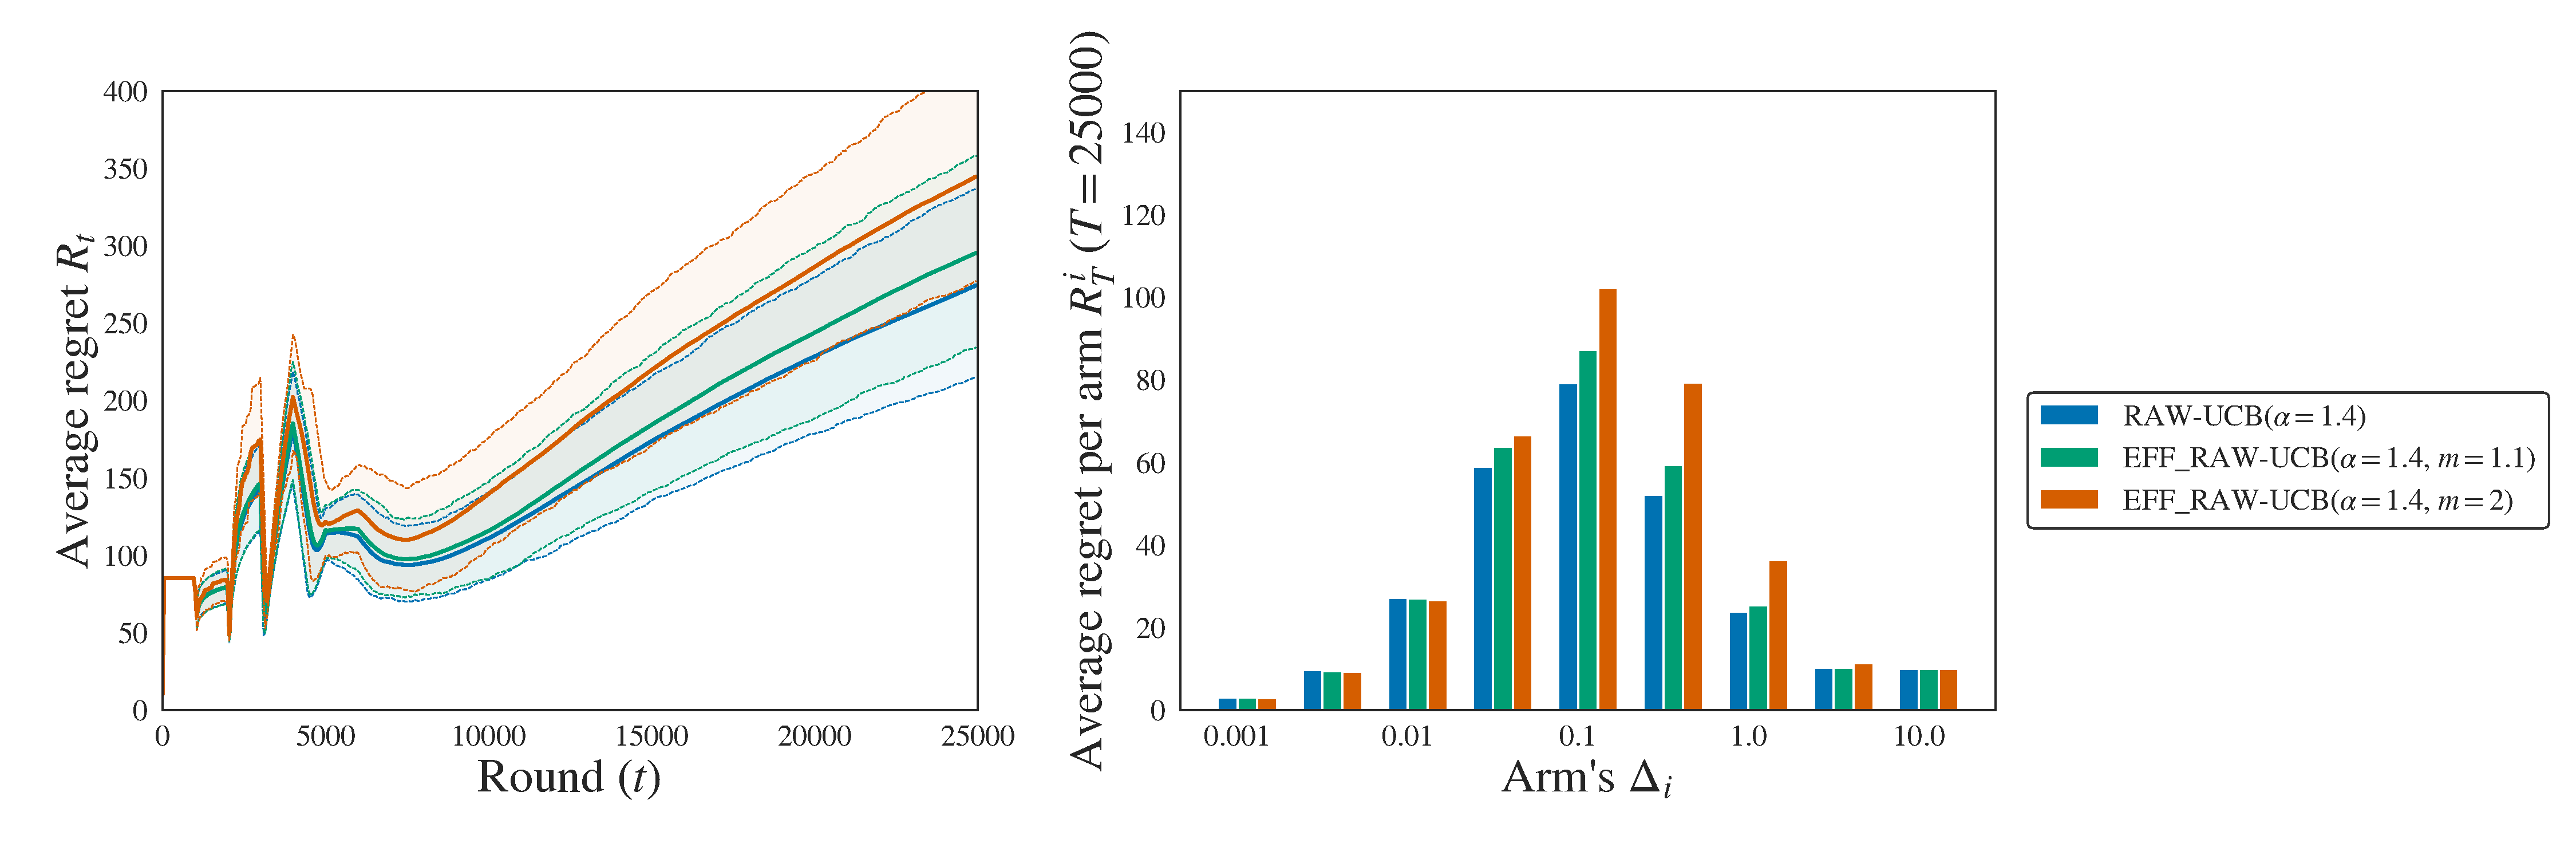
\includegraphics[width = 0.99 \textwidth]{2.1Rested/fig/fig2_eff.pdf}
\caption{\textbf{Left:} Regret at the end of the game for different values of $L$. \textbf{Middle, Right:} Regret across time for two values of $L$. Average over 1000 runs. We highlight the $\left[10\%, 90\%\right]$ confidence region.}
\label{fig:rested-eff2}
\end{figure*}

Notice that the two algorithms run in 3 seconds in average\footnote{3.0 s for $m=2$, 3.3 s for $m=1.1$} versus 25 seconds for \RAWUCB and 1 second for \wSWA. It shows that \EFFRAW effectively reduces the computation cost of \RAWUCB, even for a shorter horizon.



\subsection{Conclusion}
In this section, we provide a new update scheme which keeps $\cO\pa{\log_m t}$ averages with geometrical windows sequence of parameter $m$. These averages are updated with a delay which is proportional to the window size times $\nicefrac{m-1}{m}$. We show that when we plug this efficient update scheme in our algorithms, we recover the same upper bounds as the original algorithms with a larger multiplicative constant. However, the computational complexity is considerably reduced from $\cO(T)$ to $\cO(K\log_m T)$. We also show that in practice we can recover almost the same performance as the classical algorithms but with a computational cost that is comparable with $\wSWA$.